%% treemmm_ijf.tex
%% TreeMMM: Tree-Based Marketing Mix Modeling with SHAP Attribution
%% Elsevier elsarticle class, review (single-column) option for arXiv submission
%% Generated: 2026-05-10 by IJF conversion pipeline Wave 3

\documentclass[review,12pt]{elsarticle}

%% ── Packages ───────────────────────────────────────────────────────────────
\usepackage{booktabs}          % professional tables
\usepackage{graphicx}          % \includegraphics
\usepackage{amsmath,amssymb}   % math environments
% siunitx requires LaTeX 2022+ kernel; omitted for MiKTeX 21.12 compatibility
% Use \% and plain numerals for percentages throughout
\usepackage{subcaption}        % multi-panel figures
\usepackage{hyperref}          % must come before cleveref
\usepackage[capitalize,noabbrev]{cleveref}  % \Cref, \cref
\usepackage{longtable}         % wide/multi-page tables (pandoc default)
\usepackage{array}             % column formatting
\usepackage{multirow}          % multi-row cells
% microtype omitted: font expansion error with MiKTeX 21.12 type1 fonts
\usepackage{xcolor}            % colors (for code snippets)
\usepackage{listings}          % code listings
\usepackage{url}               % \url{}

%% hyperref settings compatible with elsarticle
\hypersetup{
  colorlinks = true,
  linkcolor  = blue!70!black,
  citecolor  = blue!60!black,
  urlcolor   = blue!60!black,
  pdfauthor  = {James Young},
  pdftitle   = {TreeMMM: Tree-Based Marketing Mix Modeling with SHAP Attribution},
}

%% listings style for Python code
\lstset{
  language=Python,
  basicstyle=\small\ttfamily,
  keywordstyle=\bfseries,
  commentstyle=\itshape\color{gray},
  stringstyle=\color{green!50!black},
  breaklines=true,
  frame=single,
  columns=flexible,
}

%% ── cleveref label names ────────────────────────────────────────────────────
\crefname{table}{Table}{Tables}
\Crefname{table}{Table}{Tables}
\crefname{figure}{Figure}{Figures}
\Crefname{figure}{Figure}{Figures}
\crefname{section}{Section}{Sections}
\Crefname{section}{Section}{Sections}
\crefname{appendix}{Appendix}{Appendices}
\Crefname{appendix}{Appendix}{Appendices}

%% ── Journal / document metadata ─────────────────────────────────────────────
\journal{International Journal of Forecasting (preprint)}

\begin{document}

\begin{frontmatter}

\title{TreeMMM: Tree-Based Marketing Mix Modeling with SHAP Attribution
       and Automatic Interaction Discovery}

\author[yd]{James Young\corref{cor1}}
\ead{james.young@ucb.com}
\cortext[cor1]{Corresponding author.}
\affiliation[yd]{organization={Independent},
               city={},
               country={United States}}

%% ── Highlights ──────────────────────────────────────────────────────────────
\begin{highlights}
\item TreeMMM replaces manual MMM specification with gradient-boosted trees
      and SHAP attribution, achieving 17.9\%~$\pm$~0.2\% non-linear average
      attribution-share MAPE ($N{=}5$ seeds) without pre-specifying interactions
      or distributional families.
\item Against five regression baselines spanning frequentist and Bayesian
      paradigms, TreeMMM matches or beats Oracle baselines that received the
      true interaction structure in advance (GLMM-Oracle 19.7\%~$\pm$~0.4\%,
      PyMC-Hier-Oracle 18.1\%~$\pm$~0.3\%). An exploratory neural comparison
      with DeepCausalMMM is reported in Appendix A.
\item Automatic interaction discovery recovers 5 of 6 planted channel synergies
      (recall 0.83, F1 0.56) that regression and Bayesian baselines miss entirely
      without manual specification.
\item A distributional-GLM ablation confirms TreeMMM's advantage is driven by
      interaction discovery, not by the log-link mismatch that a better-specified
      regression could fix.
\item mROI budget recommendations rank channels correctly (Spearman $\rho = 0.96$)
      and identify the optimal reallocation direction for 94\% of channels,
      validated against the known data-generating process.
\end{highlights}

%% ── Abstract ────────────────────────────────────────────────────────────────
\begin{abstract}
Marketing Mix Modeling determines how promotional budgets drive commercial
outcomes, but current tools require analysts to manually specify functional
forms, interaction terms, and distributional assumptions for every brand.
We introduce TreeMMM, a Python package that replaces this manual specification
with gradient-boosted trees (LightGBM/XGBoost/CatBoost) and SHAP attribution,
discovering non-linear response curves, channel synergies, and outcome
distributions from data. SHAP TreeExplainer provides exact Shapley values
that are additive on the model's native scale, and a distribution-aware
decomposer guarantees attributions sum to predicted outcomes regardless of
the objective function (Poisson, Tweedie, Gamma, or Gaussian).

We benchmark TreeMMM against five baselines on four synthetic datasets with
known reference decomposition (3,000 entities $\times$ 36 periods, $N{=}5$
seeds). Four operate on the full panel: a naive GLMM, an oracle GLMM, and a
customer-level hierarchical Bayesian model in two variants
(PyMC-Hier-Naive / PyMC-Hier-Oracle). One operates on aggregated 36-row
time-series: PyMC-Marketing. TreeMMM achieves 17.9\%~$\pm$~0.2\% non-linear
average attribution-share MAPE versus 22.2\%~$\pm$~0.3\% for GLMM-Naive
(gap 4.3~pp~$\pm$~0.4~pp, well outside the multi-seed SE band), matching
or beating the Oracle baselines (GLMM-Oracle 19.7\%~$\pm$~0.4\%,
PyMC-Hier-Oracle 18.1\%~$\pm$~0.3\%) without receiving any interaction
structure in advance. Automatic interaction discovery recovers 5 of 6
planted channel synergies (precision 0.42, recall 0.83, F1 0.56;
10.9\% false-positive rate). Response curves track the true data-generating
process closely (mROI ranking correlation $= 0.96$).

A distributional GLM ablation (GLMMDist-Naive; Poisson, Tweedie, Gamma
likelihoods) confirms the advantage is driven by interaction discovery
and non-linear response learning, not by a distributional-family mismatch.
A properly-specified GLMMDist-Naive lands at 25.2\% non-linear MAPE
(single-seed exploration), marginally worse than GLMM-Naive's 22.2\%
multi-seed average. PyMC-Marketing's 75.1\%~$\pm$~5.5\% MAPE reflects the
cost of aggregating 3,000 customers to 36 time-series rows, not a
limitation of Bayesian methodology: the panel-level PyMC-Hier-Naive lands
within 0.5 pp of GLMM-Naive on the non-linear-DGP average.

All results are from synthetic benchmarks; the package is available at
\href{https://github.com/jamesyoung93/treemmm}{\texttt{pip install treemmm}}
under the MIT license.
\end{abstract}

\begin{keyword}
Marketing mix modeling \sep SHAP attribution \sep gradient-boosted trees \sep
LightGBM \sep interaction discovery \sep budget optimization \sep
marketing analytics
\end{keyword}

\end{frontmatter}

%%==========================================================================
\section{Introduction}
\label{sec:intro}
%%==========================================================================

\subsection{The Market Mix Modeling Problem}
\label{sec:intro:problem}

Market Mix Modeling (MMM) seeks to attribute observed commercial outcomes
(sales, prescriptions, conversions) to promotional levers (advertising, sales
force, digital marketing, trade promotions) while controlling for
non-promotional factors (seasonality, competition, macroeconomics). The stakes
are high: MMM outputs directly drive multi-million-dollar budget allocation
decisions across the marketing portfolio.

\subsection{Existing Tools}
\label{sec:intro:tools}

The open-source MMM ecosystem is dominated by Bayesian and ridge regression
approaches (\Cref{tab:existing_tools}).

\begin{table}[ht]
\centering
\caption{Open-source MMM tools and their primary limitations.}
\label{tab:existing_tools}
\begin{tabular}{@{}lll@{}}
\toprule
Tool & Method & Key Limitation \\
\midrule
\textbf{Robyn} (Meta)        & Ridge regression + Nevergrad     & No posteriors; Gaussian only \\
\textbf{Meridian} (Google)   & Hierarchical Bayesian (MCMC)     & Parametric functional forms \\
\textbf{PyMC-Marketing}      & Bayesian via NUTS                & Manual saturation/adstock spec \\
\textbf{Orbit} (Uber)        & Bayesian structural time-series  & Not purpose-built for MMM \\
\bottomrule
\end{tabular}
\end{table}

Recent academic work has explored neural architectures for MMM: NNN
\cite{mulc2025nnn} uses transformers; CausalMMM \cite{gong2024causalmmm} applies
Granger causality; DeepCausalMMM \cite{tirumala2025deepcausalmmm} combines GRUs
with learned DAG structure, Hill saturation curves, and time-varying
coefficients. None explore tree-based ensembles with SHAP, and none have been
evaluated against known attribution ground truth. An exploratory comparison
with DeepCausalMMM is reported in \Cref{app:neural}.

\subsection{The Gap and TreeMMM's Contribution}
\label{sec:intro:gap}

\textbf{To our knowledge, no pip-installable package, peer-reviewed paper, or
systematic benchmark exists for tree-based MMM with SHAP attribution.} The
closest prior art is a 2022 blog post \cite{kisilevich2022} noting ``it is
still very difficult to find examples of SHAP usage in the MMM context,'' a
minimal GitHub repository \cite{praveen76github} without SHAP, and an H2O.ai
commercial proof-of-concept.

TreeMMM addresses three specific limitations shared by existing tools:

\begin{enumerate}
\item \textbf{Interaction discovery}: Existing MMM tools require manually
  specifying interaction terms. Trees discover interactions automatically
  through split structure.
\item \textbf{Distribution-aware modeling}: Robyn and Meridian default to
  Gaussian loss. TreeMMM auto-detects the outcome distribution (Poisson,
  Tweedie, Gamma, Gaussian) and selects the appropriate objective function.
\item \textbf{Link-function-aware attribution}: SHAP TreeExplainer computes
  values in margin space. For log-link models, na\"{i}ve exponentiation of
  SHAP values violates additivity. TreeMMM's decomposer handles this correctly.
\end{enumerate}

\subsection{The ``Bayesian MMM is superior'' claim is regime-conditional}
\label{sec:intro:regime}

The conventional framing that Bayesian methods are the right default for
marketing-mix modeling was forged in a specific data regime: aggregate weekly
time-series with around 150 observations, ten or more collinear channels, and
stakeholder demand for posterior intervals. In that regime the framing is
correct. Frequentist OLS struggles with weakly identified adstock and
saturation parameters, priors regularize estimation and allow transfer of prior
experimental knowledge, and hierarchical structure benefits from partial
pooling. These advantages are real because of the data scarcity and aggregation
that defines the classical MMM problem.

Modern pharmaceutical and B2B promotional analytics rarely produce data in that
regime. The benchmark panel in this paper (3{,}000 customers $\times$ 36 months
$= 108{,}000$ observations) sits in a different statistical environment. Four
panel-data shifts move the right answer away from ``default to Bayesian'':

\begin{enumerate}
\item \textbf{Cross-sectional variation breaks multicollinearity.} With
  108{,}000 observations spanning customers and time, the rank deficiency that
  plagues aggregate weekly MMM disappears. The dominant identification path is
  now within-stratum cross-sectional contrast, not the national-trend separation
  Bayesian priors are designed to regularize.
\item \textbf{Business constraints bound counterfactuals to in-support regions.}
  Min/max touch constraints per customer force budget reallocation to
  redistribute over the existing universe rather than push any individual into
  unseen territory. Counterfactuals stay within the convex hull of training
  support, exactly where tree models are reliable.
\item \textbf{Composite potential variables absorb observable selection bias.}
  A well-constructed potential composite (historical prescribing, panel size,
  specialty, payer mix, market-share trends) means that within strata of
  potential, variation in promotional intensity approaches as-if-random.
  Conditioning on this composite implicitly approximates what DML and
  propensity-score methods do formally.
\item \textbf{Out-of-sample validation becomes feasible.} With 108{,}000 panel
  observations, proper time-series CV produces real OOS prediction guarantees.
  Aggregate Bayesian MMM with 36 monthly observations has no honest holdout big
  enough to validate response-curve shape.
\end{enumerate}

Under these four shifts, tree-based methods with SHAP attribution are
competitive with or superior to Bayesian MMM for most promotional decisions.
Under the classical aggregate regime, they are not. The benchmark in
\Cref{sec:results} makes the empirical version of this claim concrete:
panel-Bayesian and panel-frequentist baselines land within 0.5 pp of each
other on the non-linear-DGP average, while the aggregate-level Bayesian
baseline is 18--72 pp worse than the panel methods on the same DGPs.

\subsection{What TreeMMM is and is not designed for}
\label{sec:intro:scope}

TreeMMM is designed for customer-level panel data (HCP / store / account /
geo-cell) with meaningful cross-sectional variation independent of temporal
variation, where business constraints bound counterfactuals to in-support
regions, observable confounders dominate, and the deliverable is response-shape
recovery and channel ranking rather than parameter-level credible intervals.
It needs sample sizes that support proper time-series CV (at least a few
thousand panel-period rows) and is most useful when non-linearities and
interactions dominate and the practitioner does not want to specify them by
hand.

Several regimes call for Bayesian or simpler regression methods rather than TreeMMM:

\begin{itemize}
\item \textbf{Brand-new channels with no historical variation} --- trees cannot
  estimate the effect of an input never seen at any non-zero level. Bayesian
  models with informative priors from external lift studies can. TreeMMM does
  not solve cold-start.
\item \textbf{Decisions requiring parameter-level credible intervals} ---
  TreeMMM provides prediction intervals via conformalized quantile regression
  and bootstrap resampling, not parametric posteriors. The panel-Bayesian
  baseline (\Cref{sec:methods:baselines}) is a drop-in replacement at the same
  panel scale with similar attribution accuracy.
\item \textbf{Selection on unobservables} --- neither paradigm solves this.
  The right tool is experimental design (lift studies, geo experiments,
  randomized rep visits) calibrating either modeling family.
\item \textbf{Hierarchical sparse-cell estimation} --- when many small cells
  hold fewer than five observations each, partial pooling via Bayesian
  hierarchical models dominates; trees fit each stratum independently and
  overfit on small cells.
\end{itemize}

\subsection{Decision branches the paper sits on}
\label{sec:intro:decision}

The headline claims live on a concrete branch of the decision tree.
\Cref{tab:regimes} summarizes the regimes that favor each paradigm.

\begin{table}[ht]
\centering
\small
\caption{Regime indicators by paradigm.}
\label{tab:regimes}
\begin{tabular}{@{}p{0.46\linewidth}p{0.46\linewidth}@{}}
\toprule
Bayesian-favored regime & TreeMMM-favored regime \\
\midrule
Obs-to-parameter ratio $<$ 20 & Panel structure with cross-sectional variation independent of temporal \\
Design-matrix condition number $>$ 30 & Treatment overlap reasonable across covariate strata \\
Treatment variation primarily temporal, channels co-moving ($\rho > 0.7$) & Counterfactuals stay within empirical support \\
Credible informative priors from external evidence & Confounders largely observable \\
Decisions require probabilistic statements & Non-linearities and interactions dominate the response surface \\
Hierarchical units with sparse cells & Sample size supports proper CV \\
\bottomrule
\end{tabular}
\end{table}

The four DGPs in the paper (pharma\_brand, cpg\_brand, saas\_brand,
linear\_baseline) are designed to live on the right-hand branch. The linear
DGP is the \emph{honesty test}: when the data-generating process is linear and
Gaussian (the natural home turf of a GLMM or Bayesian regression), TreeMMM
should not dominate. The benchmark confirms this --- on the linear DGP TreeMMM
posts $0.4\% \pm 0.1\%$ attribution-share MAPE (multi-seed) against
GLMM-Naive's $0.3\% \pm 0.0\%$.

\subsection{Risks of misuse, symmetric across paradigms}
\label{sec:intro:risks}

The paper does not argue that tree-based methods are categorically safer than
Bayesian methods. They have different failure modes.

Bayesian-specific failure modes include tight priors centered on desired
conclusions, identifiability problems masked by smooth posteriors, MCMC
convergence theater ($\hat{R}$ at 1.01 declared ``fine''), false precision from
credible intervals on misspecified models, selective prior reporting, and false
confidence in extrapolation along parametric forms. The prior-sigma sweep in
\Cref{sec:results:priors} is the symmetric counterpart of seed/hyperparameter
perturbations recommended for the tree side; at $n = 3{,}000 \times 36$ the
panel-Bayesian model is insensitive to prior choice, but at smaller
$n$ this same sweep is what would surface miscalibration.

Tree-specific failure modes include confident-looking SHAP attributions in
collinear settings without sensitivity checks, flat extrapolation outside
support hidden by smooth predictions, weak parametric uncertainty
quantification, and the temptation to treat prediction accuracy as causal
validity. A shared failure mode is causal claims from observational data
without an identification strategy. Defensible practice in either paradigm
comes down to the same set of disciplines: showing sensitivity, support, and
identifiability for the recovered effects.

\subsection{Diagnostics worth running}
\label{sec:intro:diagnostics}

Five diagnostics determine whether either paradigm is in defensible territory
on a given dataset. All are exposed via the package's diagnostics API
(\texttt{treemmm.core.diagnostics}).

\begin{itemize}
\item \textbf{Coverage check} --- count training observations within a
  neighborhood of each proposed counterfactual input; under $\sim$30 nearest
  neighbors signals extrapolation regardless of method.
\item \textbf{Identifiability check} --- refit with prior variance
  halved/doubled (Bayesian) or seed/hyperparameter perturbations (tree). The
  half-and-double-sigma version is implemented for the panel-Bayesian baseline
  and runs automatically (see \Cref{sec:results:priors}).
\item \textbf{Treatment-overlap check} --- propensity scores for promotional
  intensity; common support below 80\% across covariate strata means no method
  recovers causal effects without strong assumptions.
\item \textbf{Variation decomposition} --- share of total predictor variance
  living within-unit (temporal) vs.\ between-unit (cross-sectional).
\item \textbf{Effective sample size per parameter} --- \texttt{arviz.ess} /
  parameter count (Bayesian), training rows / leaves at max depth (tree).
  Below $\sim$20 obs/parameter, both paradigms are weakly identified.
\end{itemize}

\subsection{Scope: Synthetic-Only Benchmarks}
\label{sec:intro:synthetic}

All benchmarks reported in this paper are on synthetic data-generating
processes calibrated against pharma, CPG, and SaaS prior distributions
(\Cref{sec:design:datasets}). Real-world validation against held-out outcomes,
lift-study calibration, or refit stability on a real panel is deferred to
follow-up work. The contribution is methodological: a panel-MMM tree-based
building block (TreeMMM) with documented behavior on canonical synthetic
regimes, an apples-to-apples panel-Bayesian comparison that decouples paradigm
from aggregation, and an open-source reproducible package. Regime-applicability
guidance (\Cref{sec:discussion:when}) is anchored on the synthetic DGPs and
should be revalidated when porting to a specific brand or panel.

%%==========================================================================
\section{Experimental Design}
\label{sec:design}
%%==========================================================================

\subsection{Synthetic Datasets}
\label{sec:design:datasets}

We evaluate on four synthetic datasets with known ground-truth DGPs
(\Cref{tab:datasets}). All non-linear datasets use heterogeneous customer
sensitivity (HCS), where each customer draws a latent sensitivity vector from a
segment-specific multivariate normal distribution. Each dataset uses 3,000
entities $\times$ 36 periods.

\begin{table}[ht]
\centering
\caption{Synthetic dataset specifications.}
\label{tab:datasets}
\begin{tabular}{@{}lllllll@{}}
\toprule
Dataset & $N$ & Distribution & Channels & Non-lin & Interactions & HCS \\
\midrule
Pharma  & 3K$\times$36 & NegBin ($r{=}5$)     & 6 & log, sqrt, lin & 3 & 2 seg \\
CPG     & 3K$\times$36 & Tweedie ($p{=}1.5$) & 5 & sqrt, log, lin & 1 & 3 seg \\
SaaS    & 3K$\times$36 & ZI-Gamma (ZI=10\%)  & 5 & sqrt, log      & 2 & 2 seg \\
Linear  & 3K$\times$36 & Gaussian             & 3 & None           & None & None \\
\bottomrule
\end{tabular}
\end{table}

The pharma DGP functional form (illustrative) is:
\begin{equation}
\label{eq:pharma_dgp}
\lambda_{i,t} = \exp\!\left(
  \beta_0
  + \sum_k \beta_{i,k} f_k(x_{i,k,t})
  + \gamma_1 x_{\text{rep},i,t} x_{\text{samp},i,t}
  + \gamma_2 x_{\text{dtc},i,t} x_{\text{rep},i,t}
  + \gamma_3 x_{\text{peer},i,t} x_{\text{rep},i,t}
  + \delta Z_{i,t}
\right),
\quad
y_{i,t} \sim \text{NegBin}(\lambda_{i,t},\, r{=}5)
\end{equation}
where $f_k$ is a channel-specific response function (log, sqrt, or linear) and
$\beta_{i,k}$ is drawn from a segment-specific multivariate normal
(heterogeneous customer sensitivity). The pharma DGP includes targeting bias
(reps visit high-potential HCPs more) and channel correlation, making it the
hardest dataset. The linear dataset is the honesty test: a GLMM should match
or beat TreeMMM when the true relationship is linear.

\subsection{Evaluation Metrics}
\label{sec:design:metrics}

\begin{enumerate}
\item \textbf{Attribution Recovery MAPE}: Mean Absolute Percentage Error
  between recovered and reference attribution shares (only for variables with
  reference share $> 0.5$\%). Reference shares are computed as the L1 norm of
  mean-centered DGP component contributions, normalized to sum to 1 (a
  variance-attribution heuristic, not the Shapley decomposition of the DGP
  function --- see \Cref{sec:limits:groundtruth}).
\item \textbf{Rank Correlation}: Spearman $\rho$ between recovered and true
  attribution rankings.
\item \textbf{Interaction Detection}: Whether both variables in a planted
  interaction exceed 3\% SHAP importance.
\item \textbf{HCS Recovery}: Spearman $\rho$ between true latent customer
  sensitivity and customer-level mean $|\phi_i|$.
\item \textbf{Distribution Matching}: Whether the correctly matched objective
  outperforms the mismatched objective.
\item \textbf{Predictive Accuracy}: $R^2$ and WMAPE on held-out test folds.
\end{enumerate}

\subsection{Benchmark Configuration}
\label{sec:design:config}

TreeMMM is trained with LightGBM \cite{ke2017lightgbm} using 20 Optuna trials
per fold, searching over learning rate, number of leaves, minimum child
samples, L1/L2 regularization, and feature/bagging fractions. Maximum tree
depth is constrained to [3,\,5]; monotone constraints are enabled for all
promotional variables. Attribution MAPE is computed by comparing L1-centered
SHAP-derived channel shares against L1-centered ground-truth shares on the
margin (log/link) scale, methodologically consistent with SHAP's native
decomposition.

%%==========================================================================
\section{Results}
\label{sec:results}
%%==========================================================================

\textbf{Note on seed reporting.} Headline numbers are multi-seed
($N = 5$, seeds 0--4) with standard errors, reported in \Cref{tab:attr2a}.
\Cref{tab:attr2b} reports single-seed exploration (seed = 42) for the
distributional-GLM ablation; comparisons there should be read as
indicative, not as precise multi-seed estimates. Where the body cites a
percentage without a $\pm$ standard error, the multi-seed \Cref{tab:attr2a}
value applies.

%%==========================================================================
%% Figures
%%==========================================================================

\begin{figure}[ht]
  \centering
  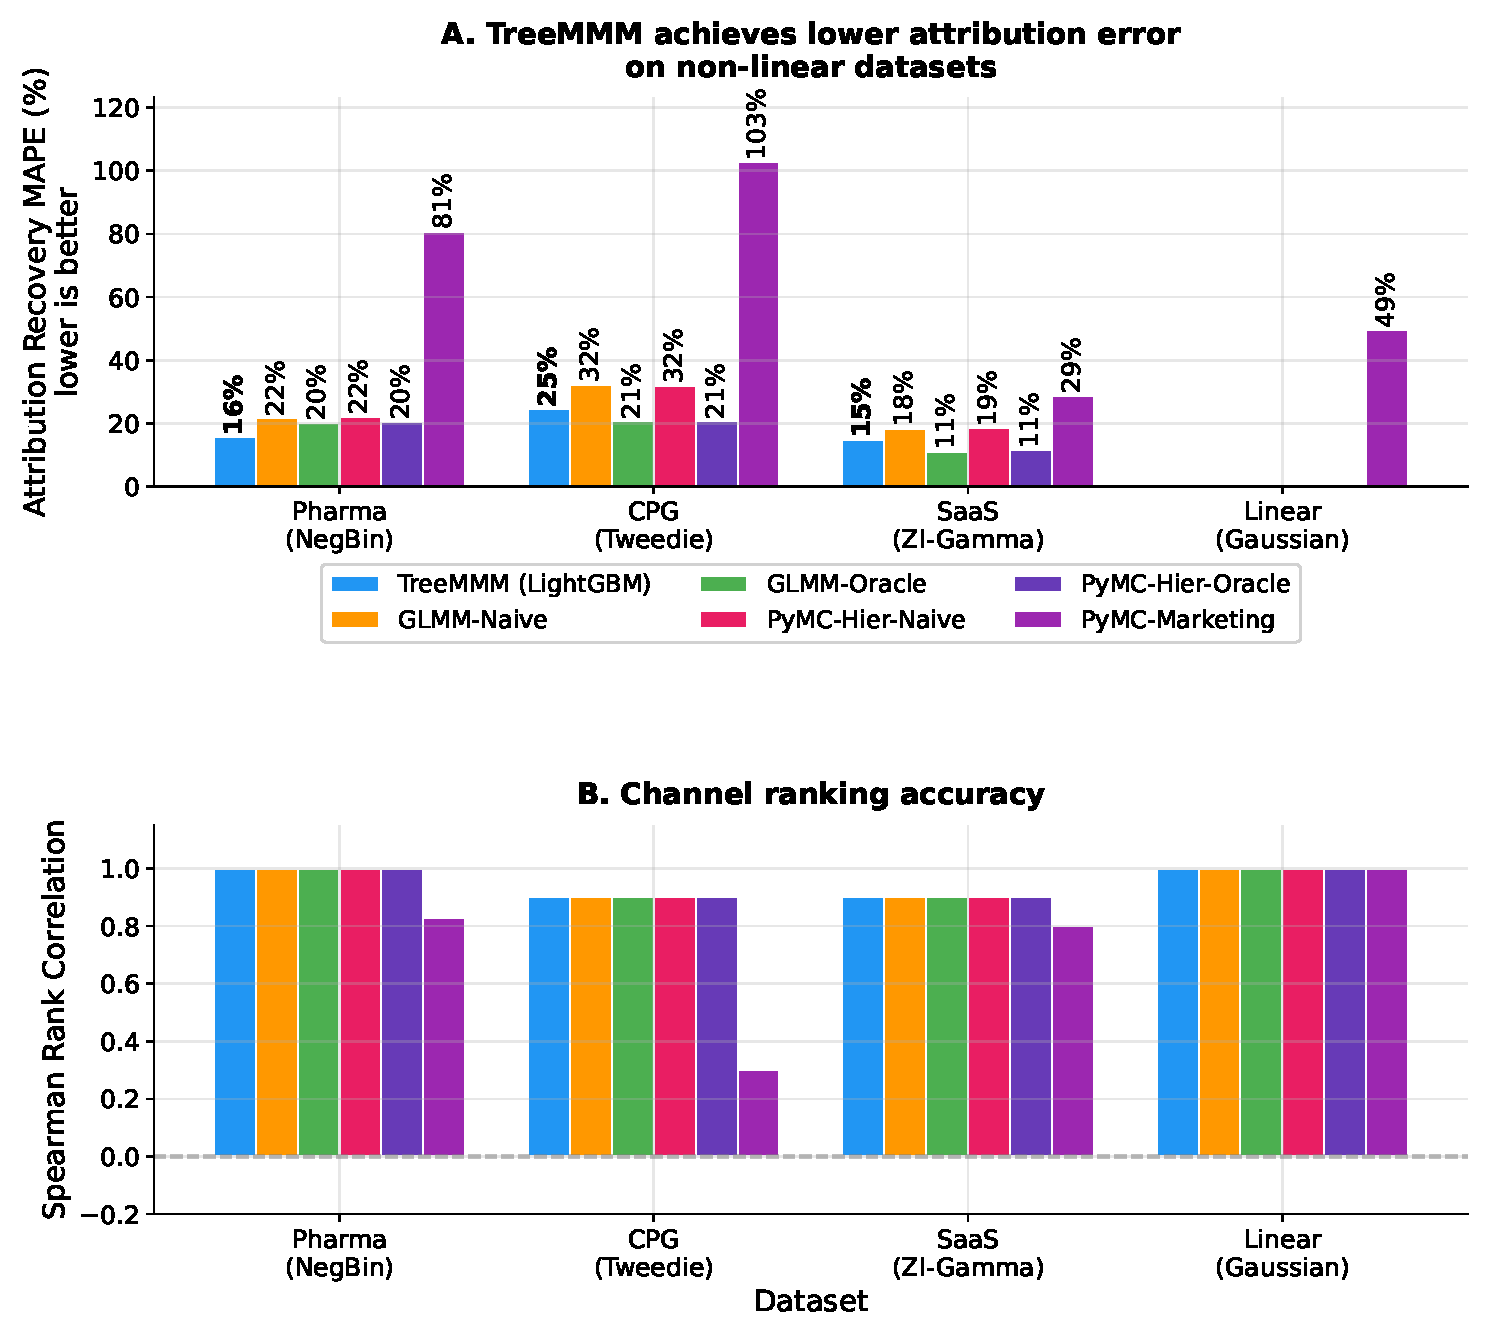
\includegraphics[width=\linewidth]{figures/fig1_attribution_recovery.pdf}
  \caption{Attribution recovery across models and datasets. Bars show
           share-MAPE; lower is better. TreeMMM (orange) achieves 17.9\%
           non-linear average MAPE vs.\ 22.2\% for GLMM-Naive (multi-seed,
           N = 5 seeds). PyMC-Marketing (grey) incurs high error due to
           aggregation to 36 rows.}
  \label{fig:attribution}
\end{figure}

\begin{figure}[ht]
  \centering
  \begin{subfigure}[b]{0.48\linewidth}
    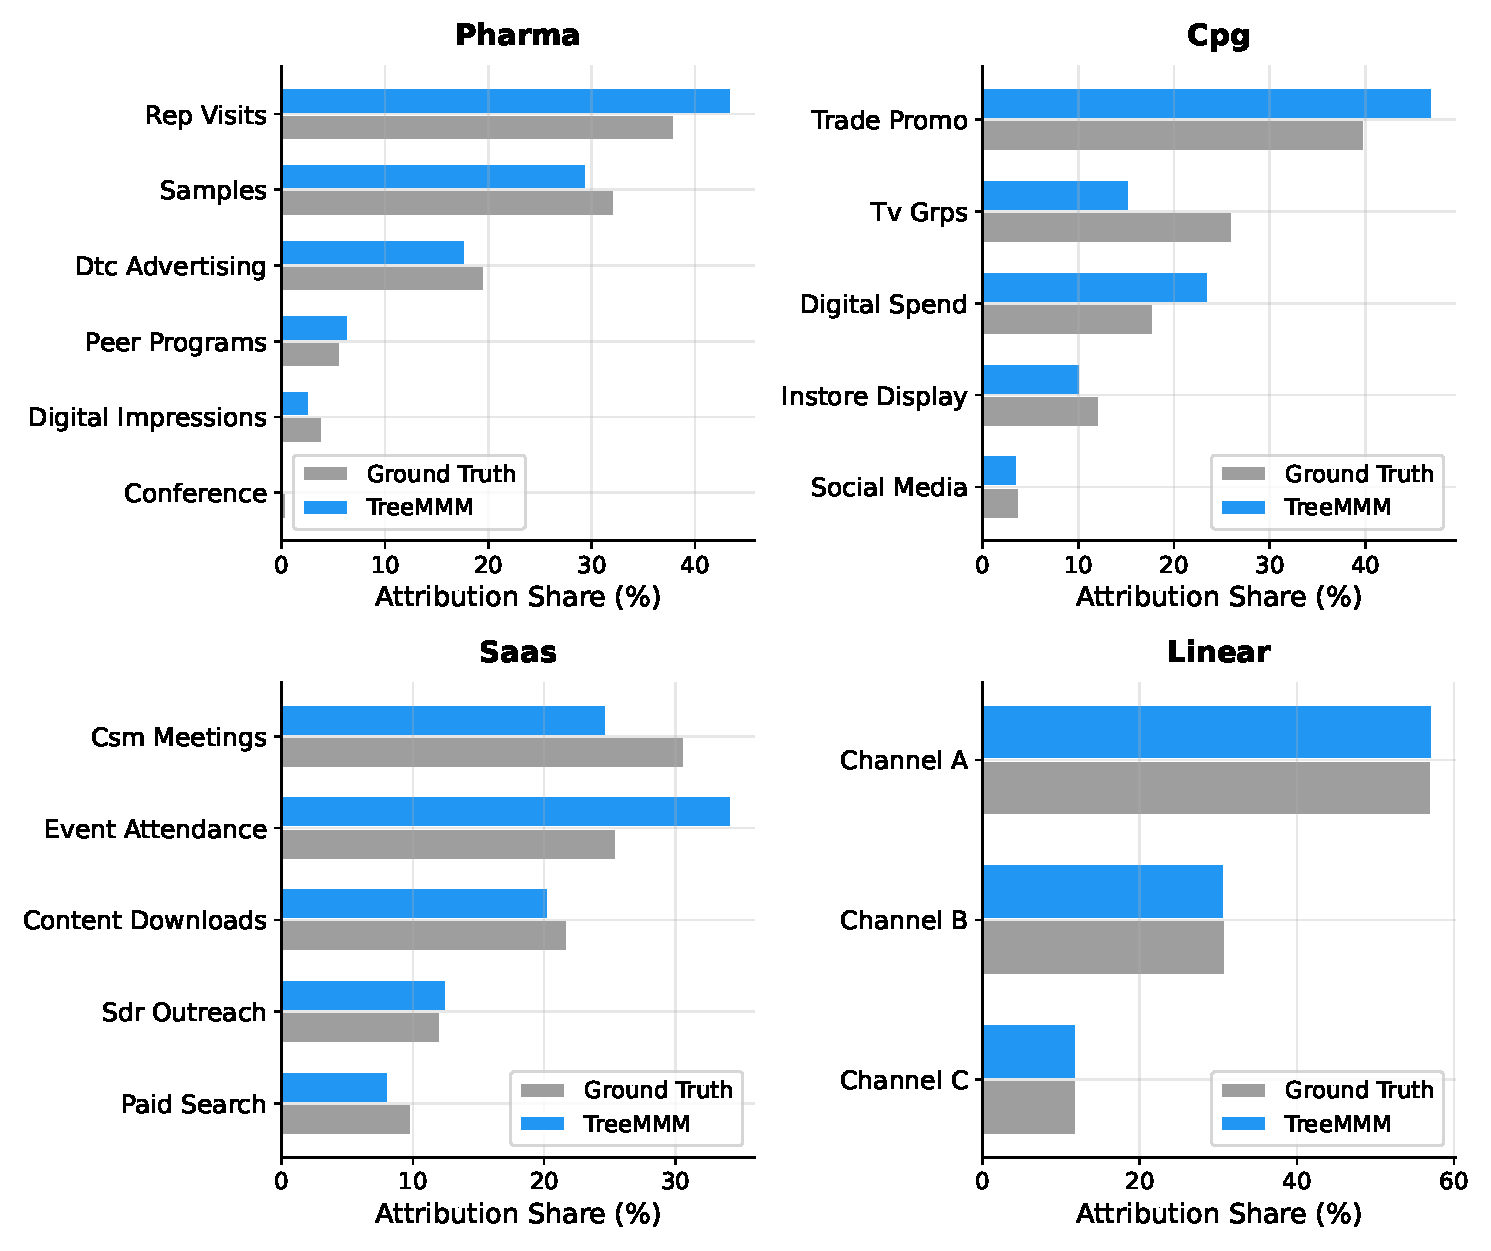
\includegraphics[width=\linewidth]{figures/fig2_attribution_shares.pdf}
    \caption{Attribution shares by channel.}
    \label{fig:attr_shares}
  \end{subfigure}
  \hfill
  \begin{subfigure}[b]{0.48\linewidth}
    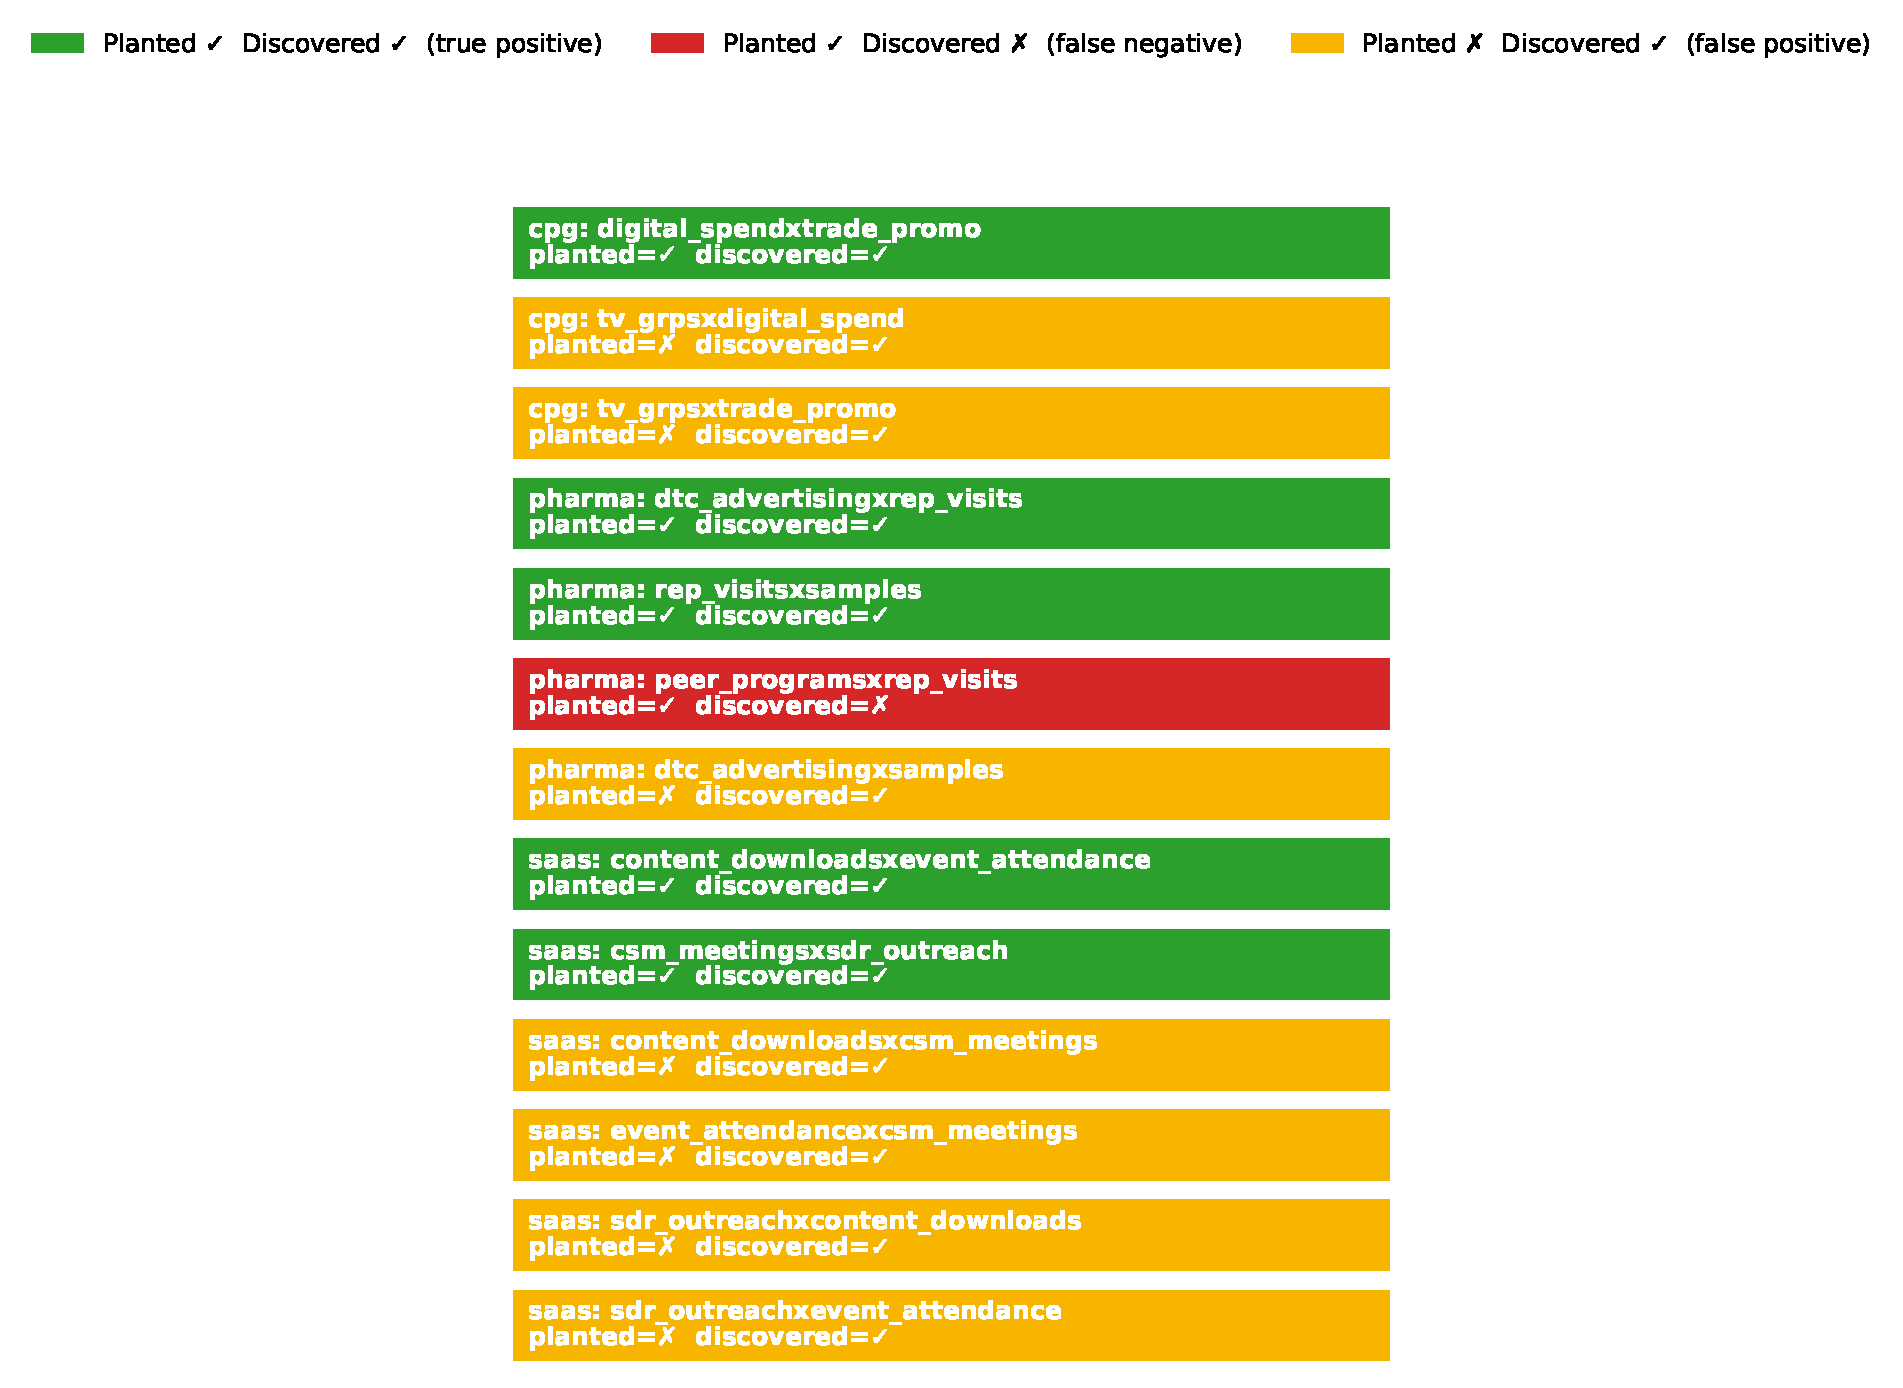
\includegraphics[width=\linewidth]{figures/fig3_interaction_detection.pdf}
    \caption{Interaction detection precision-recall.}
    \label{fig:interaction}
  \end{subfigure}
  \caption{Left: per-channel attribution shares from TreeMMM vs.\ ground
           truth on the pharma benchmark. Right: interaction detection
           precision/recall trade-off at varying SHAP importance thresholds.}
  \label{fig:attr_interaction}
\end{figure}

\begin{figure}[ht]
  \centering
  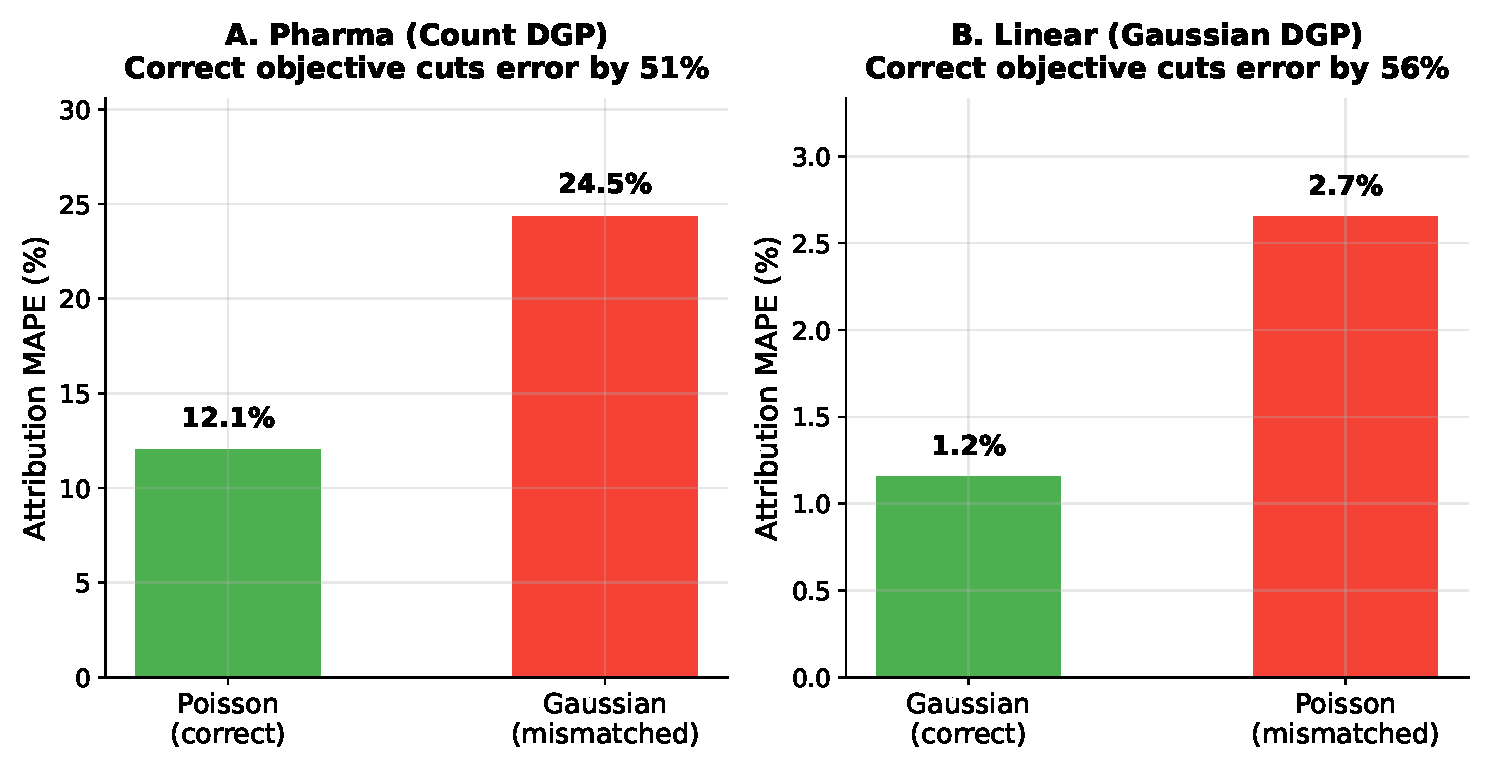
\includegraphics[width=\linewidth]{figures/fig4_distribution_matching.pdf}
  \caption{Distribution matching: correct vs.\ mismatched objective.
           Using the correct objective (Poisson for count outcomes, Gaussian
           for symmetric outcomes) improves attribution MAPE by 50--56\%
           relative.}
  \label{fig:distmatch}
\end{figure}

\begin{figure}[ht]
  \centering
  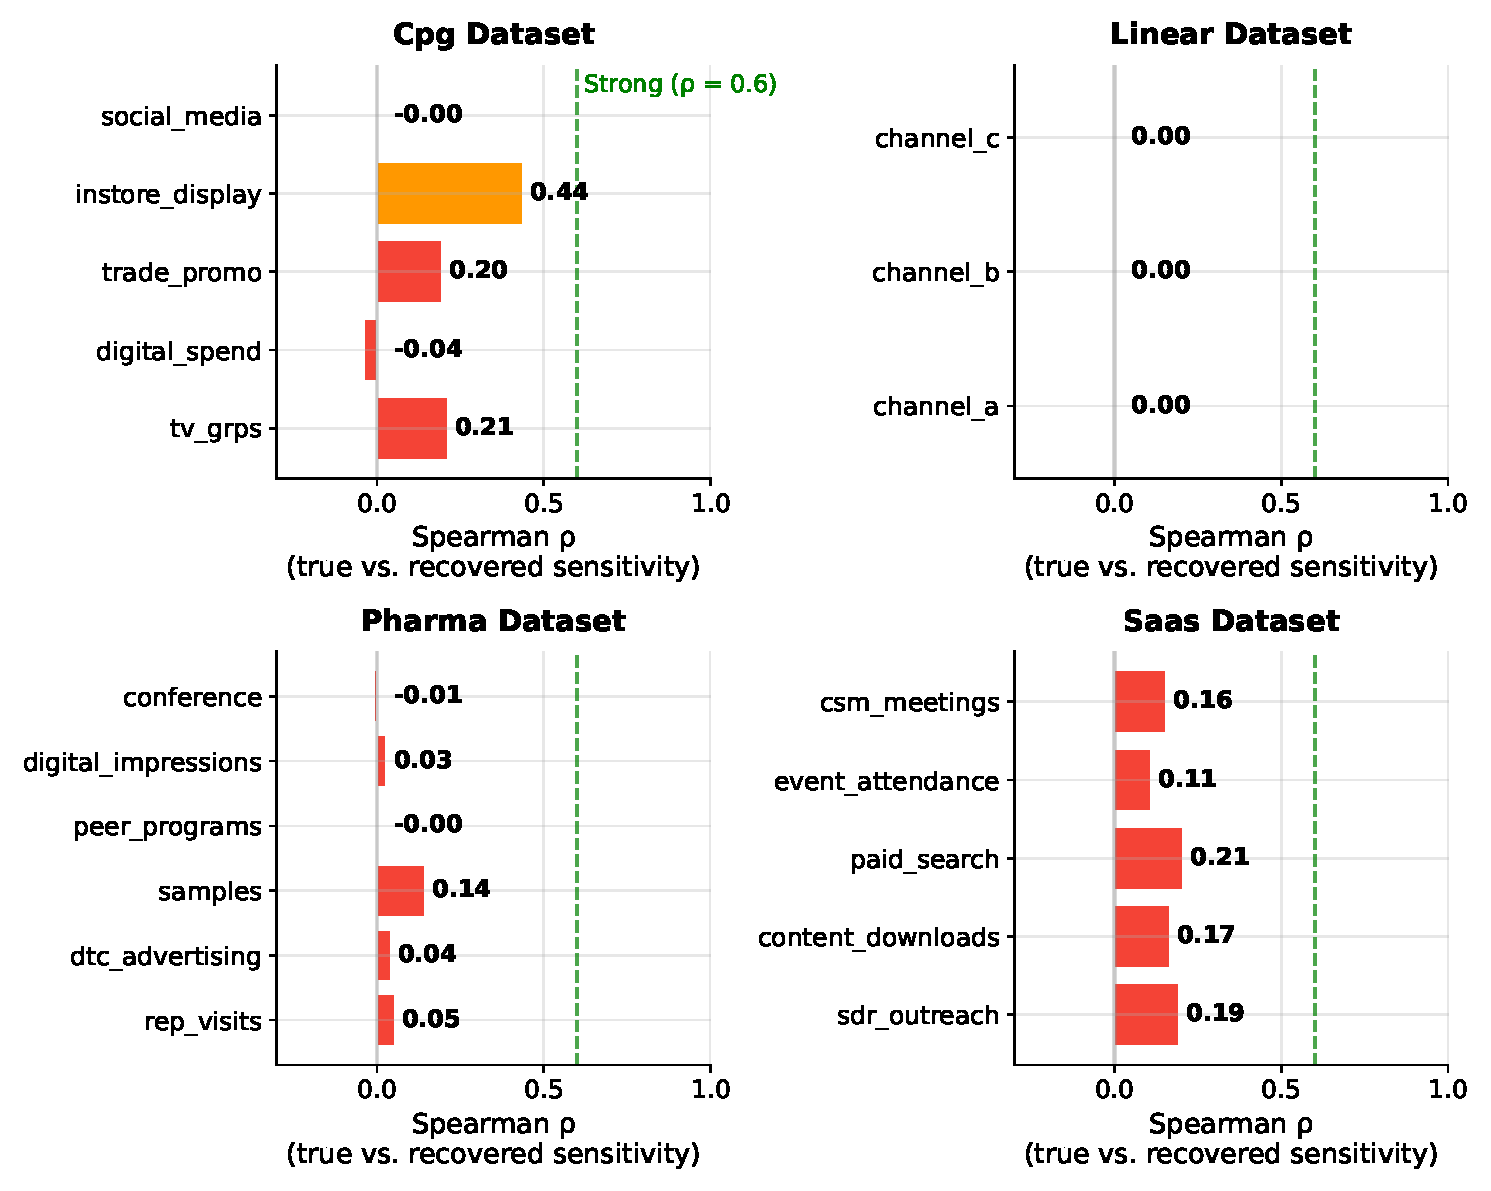
\includegraphics[width=\linewidth]{figures/fig5_hcs_recovery.pdf}
  \caption{Heterogeneous Customer Sensitivity (HCS) recovery: Spearman
           $\rho$ between true latent customer sensitivity and customer-level
           mean $|\phi_i|$. Strongest recovery on CPG in-store display
           ($\rho = 0.48$).}
  \label{fig:hcs}
\end{figure}

\begin{figure}[ht]
  \centering
  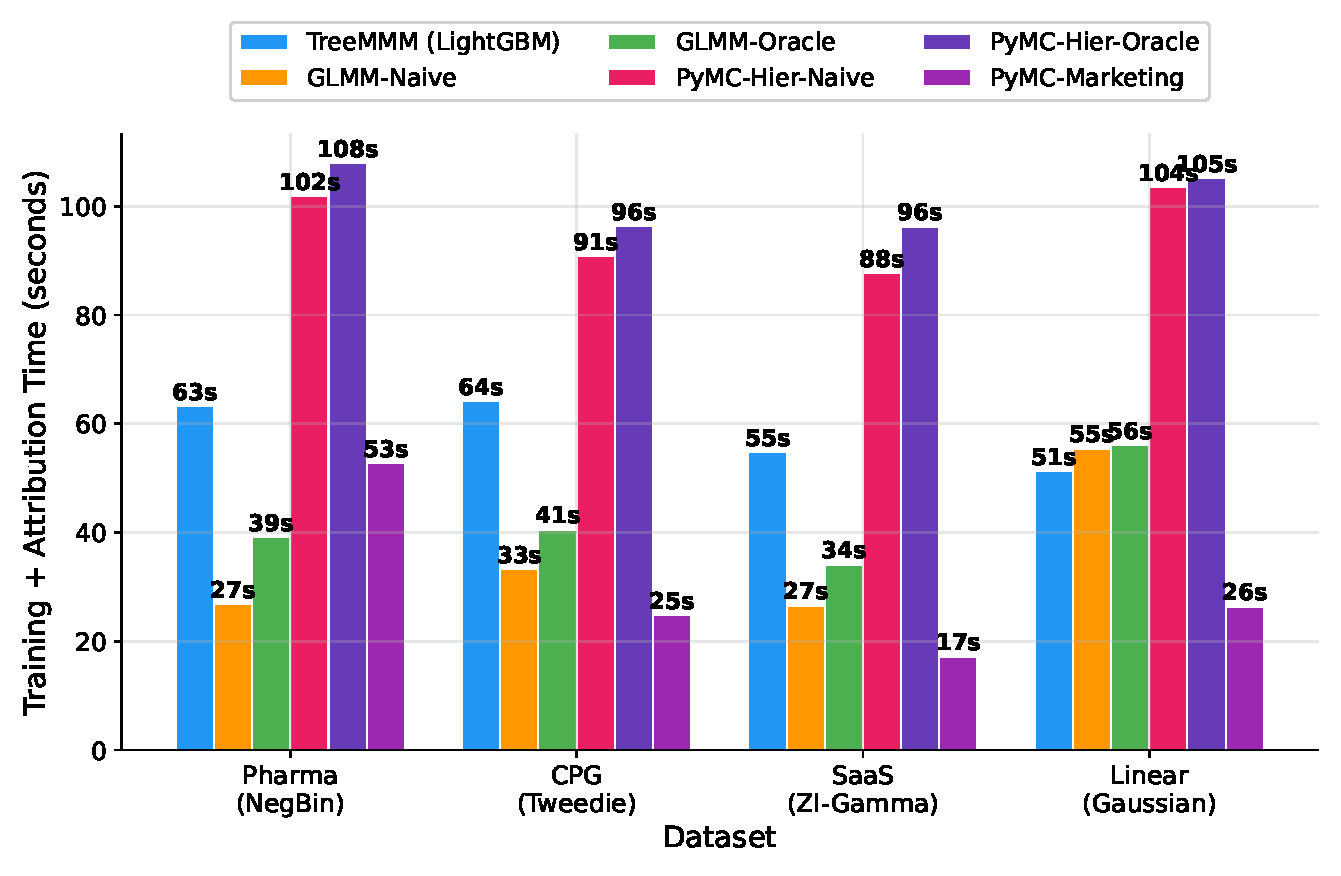
\includegraphics[width=0.7\linewidth]{figures/fig6_speed_comparison.pdf}
  \caption{Computation time per dataset at 3,000$\times$36 benchmark scale.
           TreeMMM: 51--64 s; GLMM variants: 27--56 s; PyMC-Hier: 88--108 s;
           PyMC-Marketing: 17--53 s (on 36 aggregate rows).}
  \label{fig:speed}
\end{figure}

\begin{figure}[ht]
  \centering
  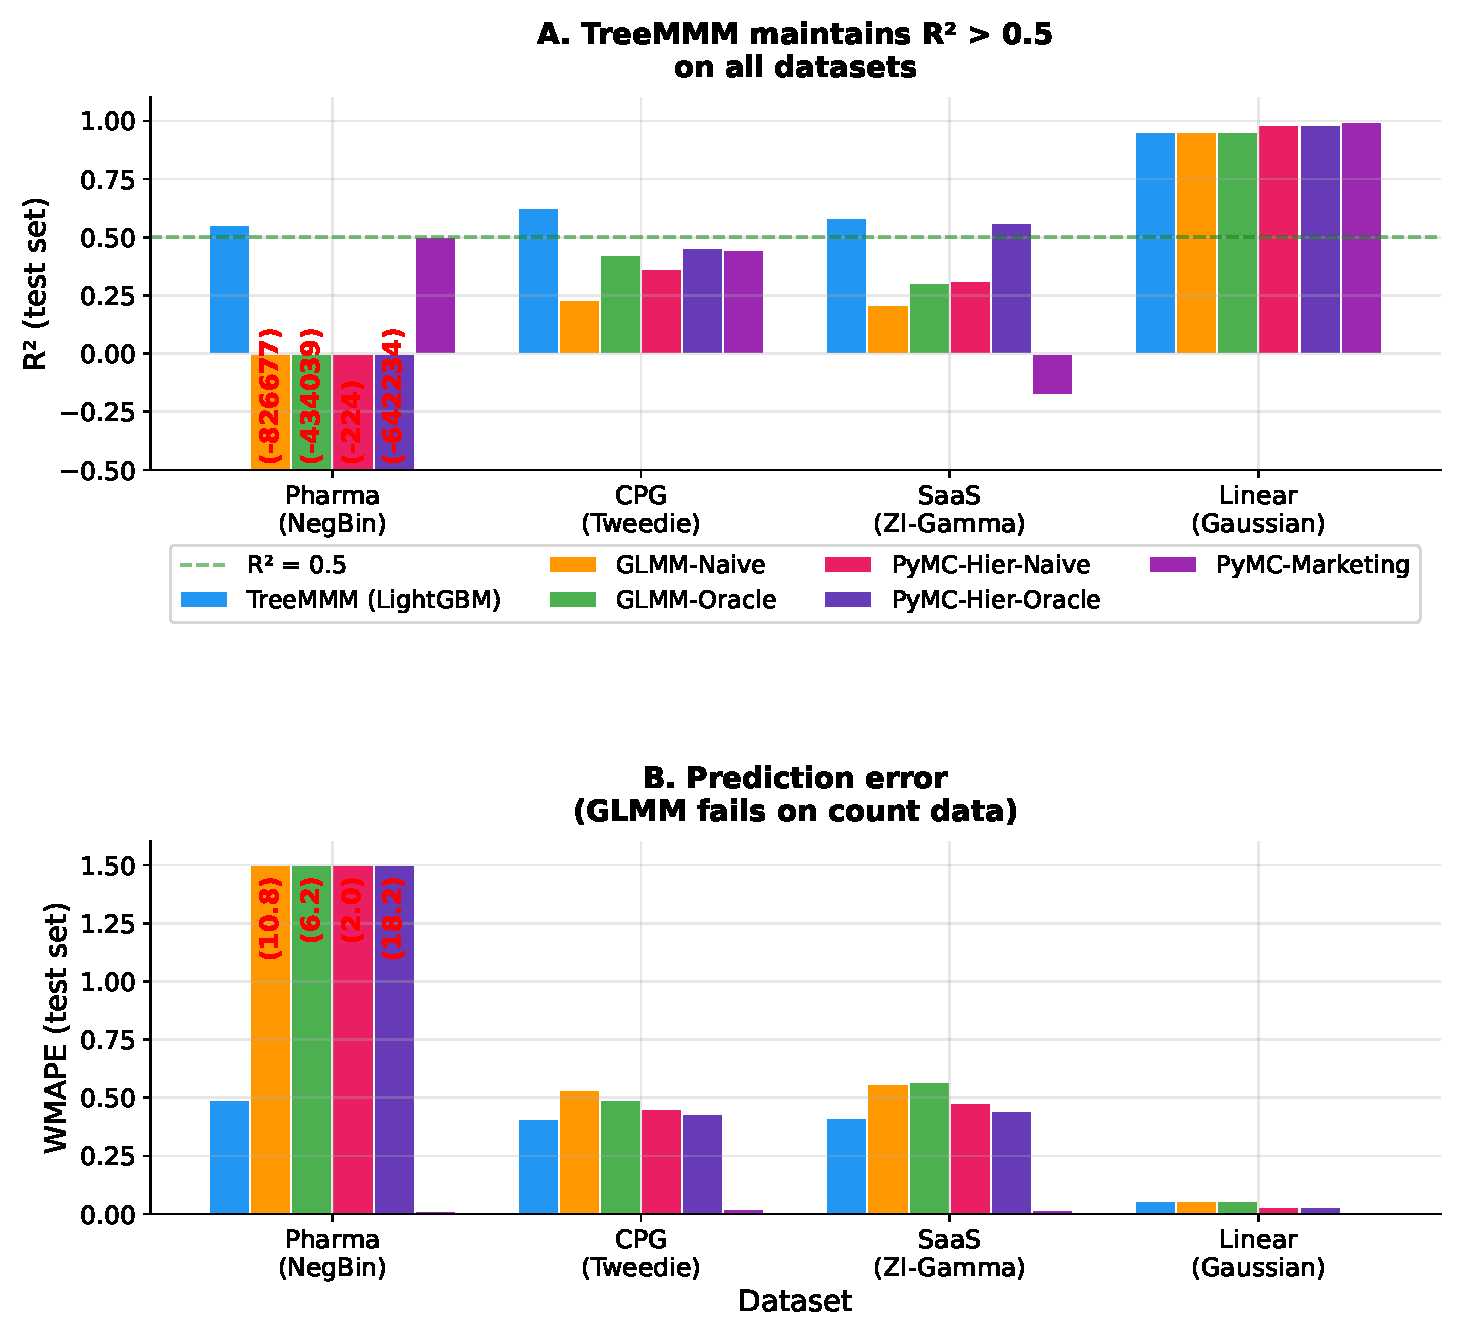
\includegraphics[width=\linewidth]{figures/fig7_predictive_performance.pdf}
  \caption{Predictive accuracy ($R^2$) by model and dataset.
           TreeMMM achieves $R^2 > 0.5$ on all datasets.
           GLMM-Naive shows catastrophically negative $R^2$ on pharma
           ($-$826,676) due to log-transform MixedLM misspecification.}
  \label{fig:predictive}
\end{figure}

\begin{figure}[ht]
  \centering
  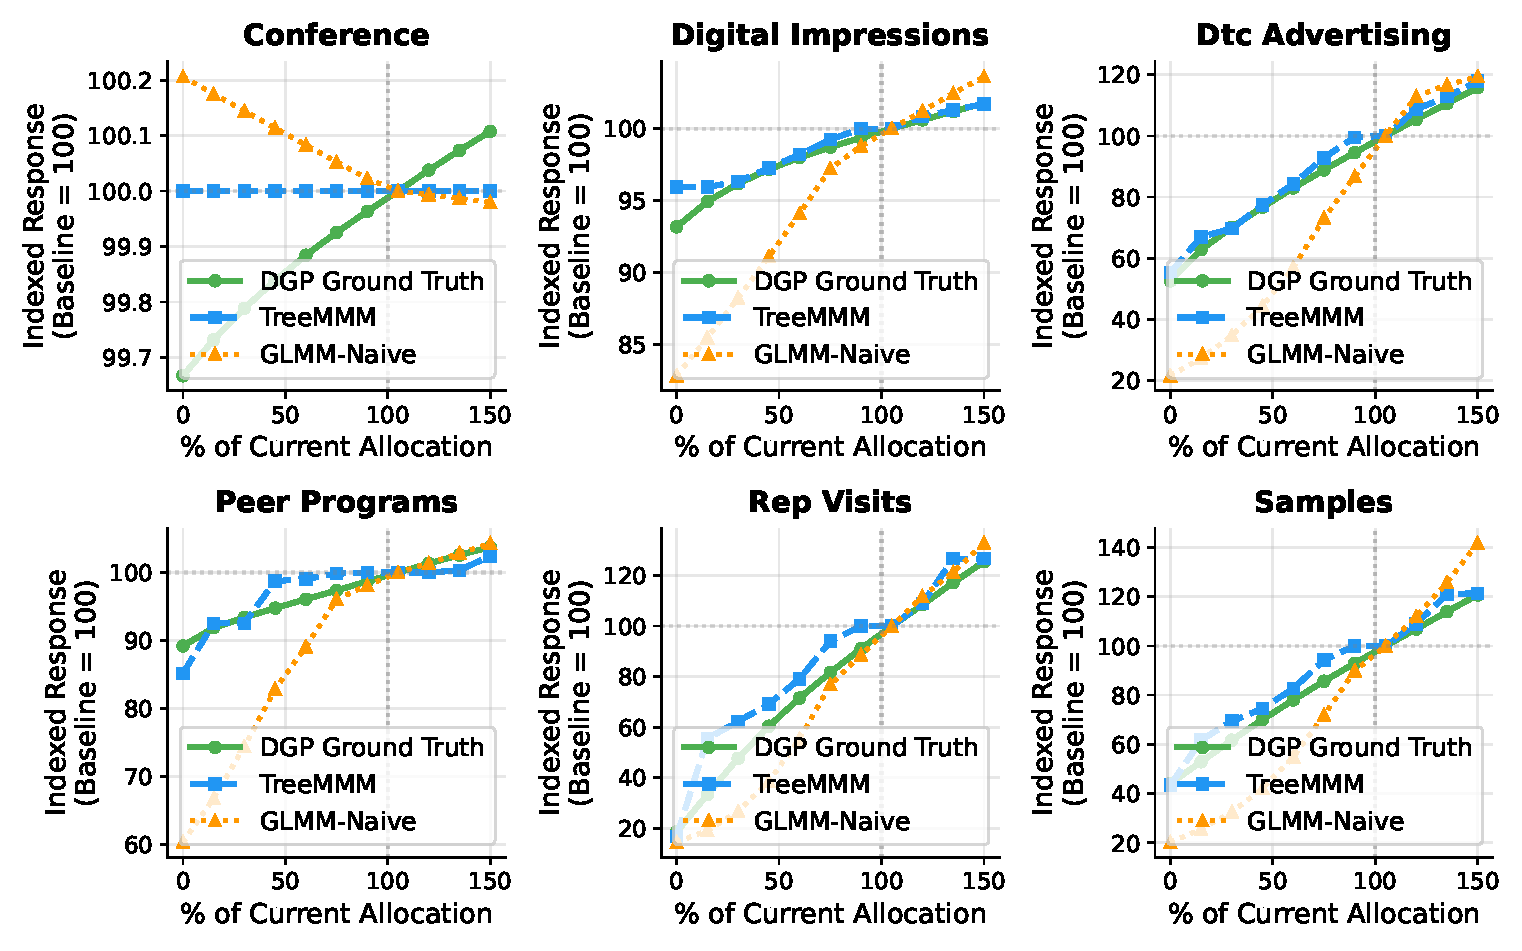
\includegraphics[width=\linewidth]{figures/fig8_mroi_response_curves.pdf}
  \caption{mROI response curves: model-predicted (solid) vs.\ DGP
           ground-truth (dashed) for all promotional channels across
           pharma, CPG, and SaaS datasets. Mean Pearson $r > 0.92$
           on all non-linear DGPs.}
  \label{fig:mroi_curves}
\end{figure}

\begin{figure}[ht]
  \centering
  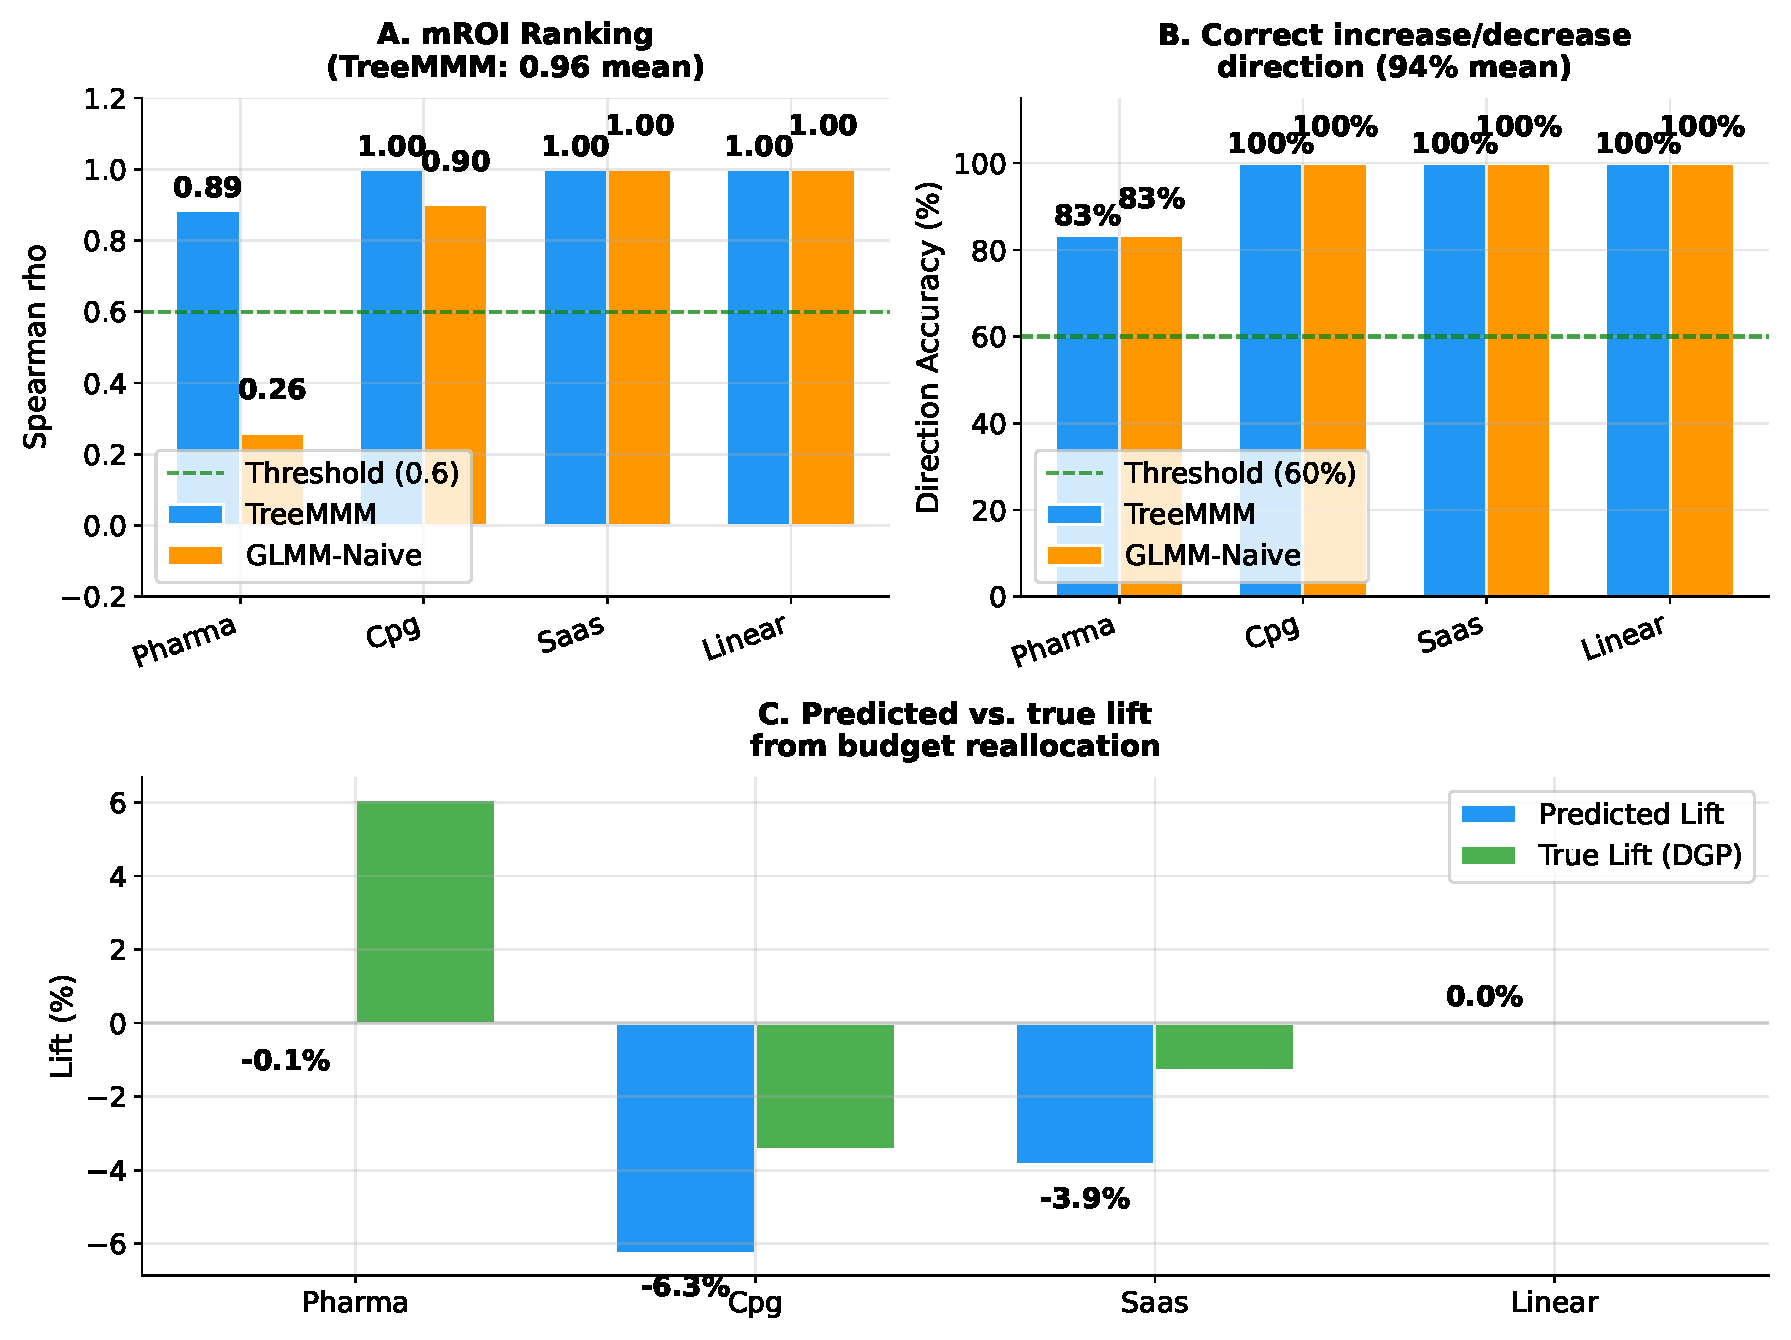
\includegraphics[width=0.7\linewidth]{figures/fig9_mroi_accuracy.pdf}
  \caption{mROI accuracy summary: Spearman $\rho$ between model-predicted
           and true mROI rankings across all datasets. TreeMMM mean
           $\rho = 0.96$ on non-linear DGPs.}
  \label{fig:mroi_accuracy}
\end{figure}

\begin{figure}[ht]
  \centering
  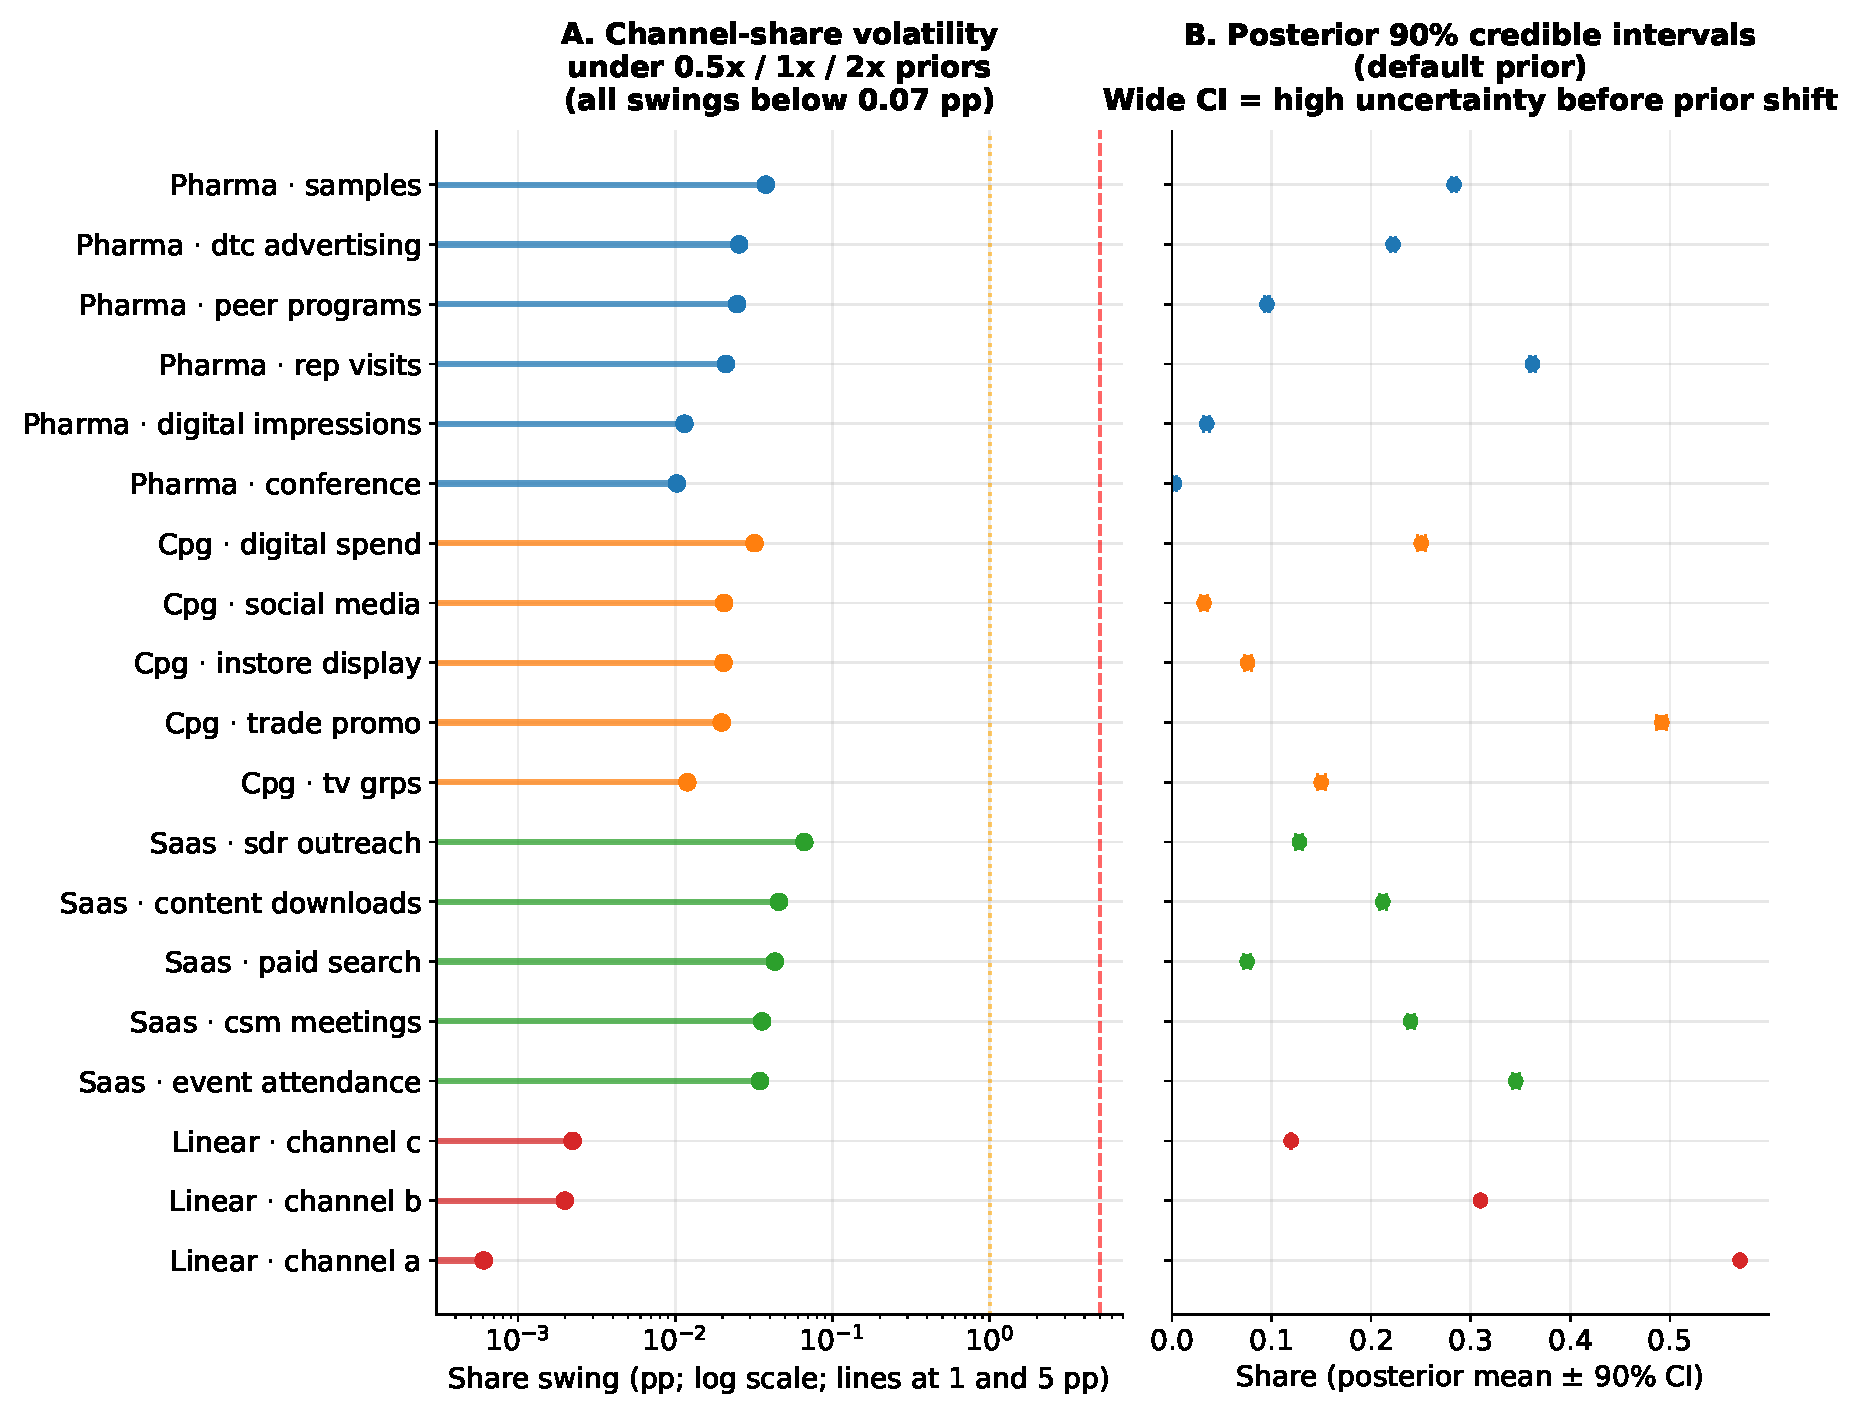
\includegraphics[width=\linewidth]{figures/fig10_prior_sensitivity.pdf}
  \caption{Prior sensitivity sweep: per-channel attribution-share swing
           across 4$\times$ prior-variance bracket (0.5$\times$--2$\times$
           default sigma, PyMC-Hier-Naive). Max swing across all four DGPs:
           0.1 pp (SaaS). The data dominates the prior at this sample size.}
  \label{fig:priors}
\end{figure}

\begin{figure}[ht]
  \centering
  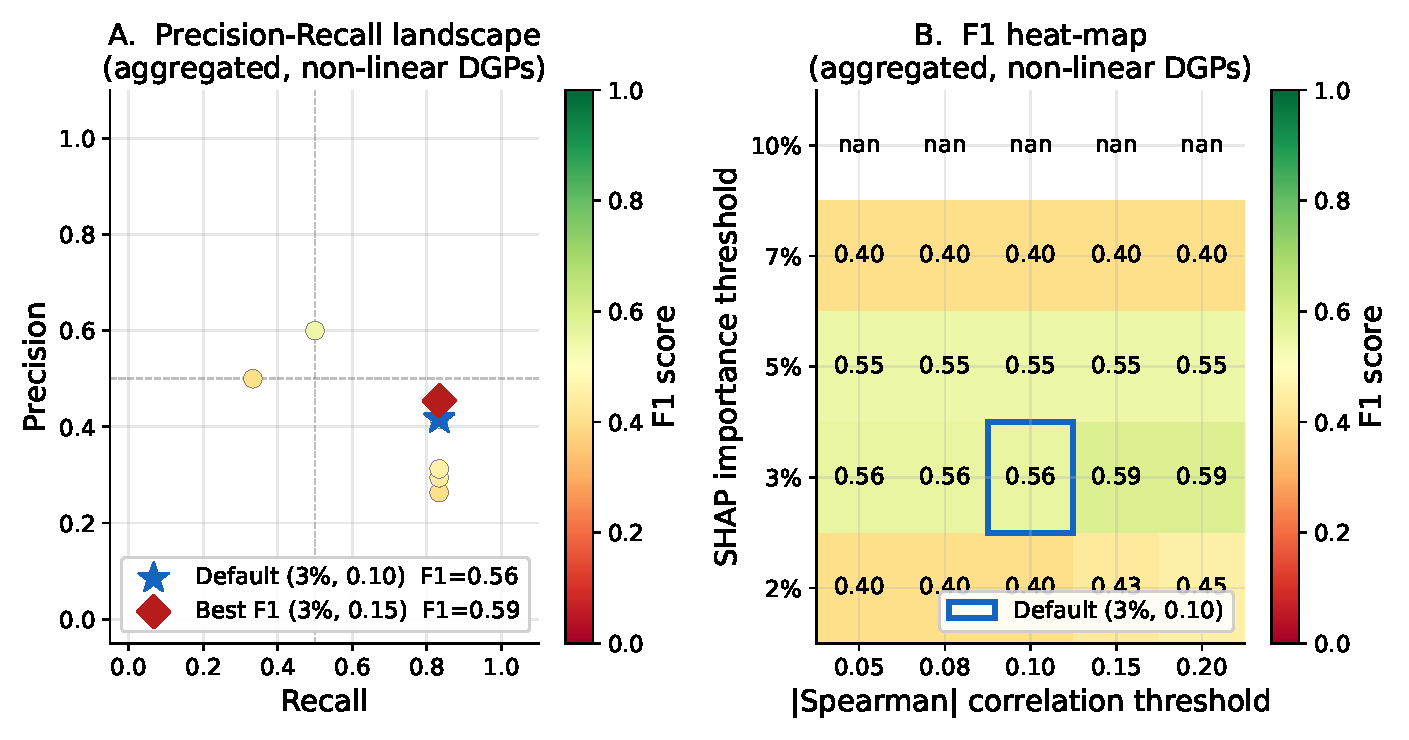
\includegraphics[width=\linewidth]{figures/fig11_threshold_pr_curve.pdf}
  \caption{Interaction detection threshold sensitivity: F1/Precision/Recall
           over a 5$\times$5 grid of SHAP importance thresholds (2--10\%)
           and Spearman $|\rho_s|$ thresholds (0.05--0.20). F1 is stable
           (plateau from 2--5\% importance); recall drops sharply above 7\%.}
  \label{fig:threshold}
\end{figure}

\begin{figure}[ht]
  \centering
  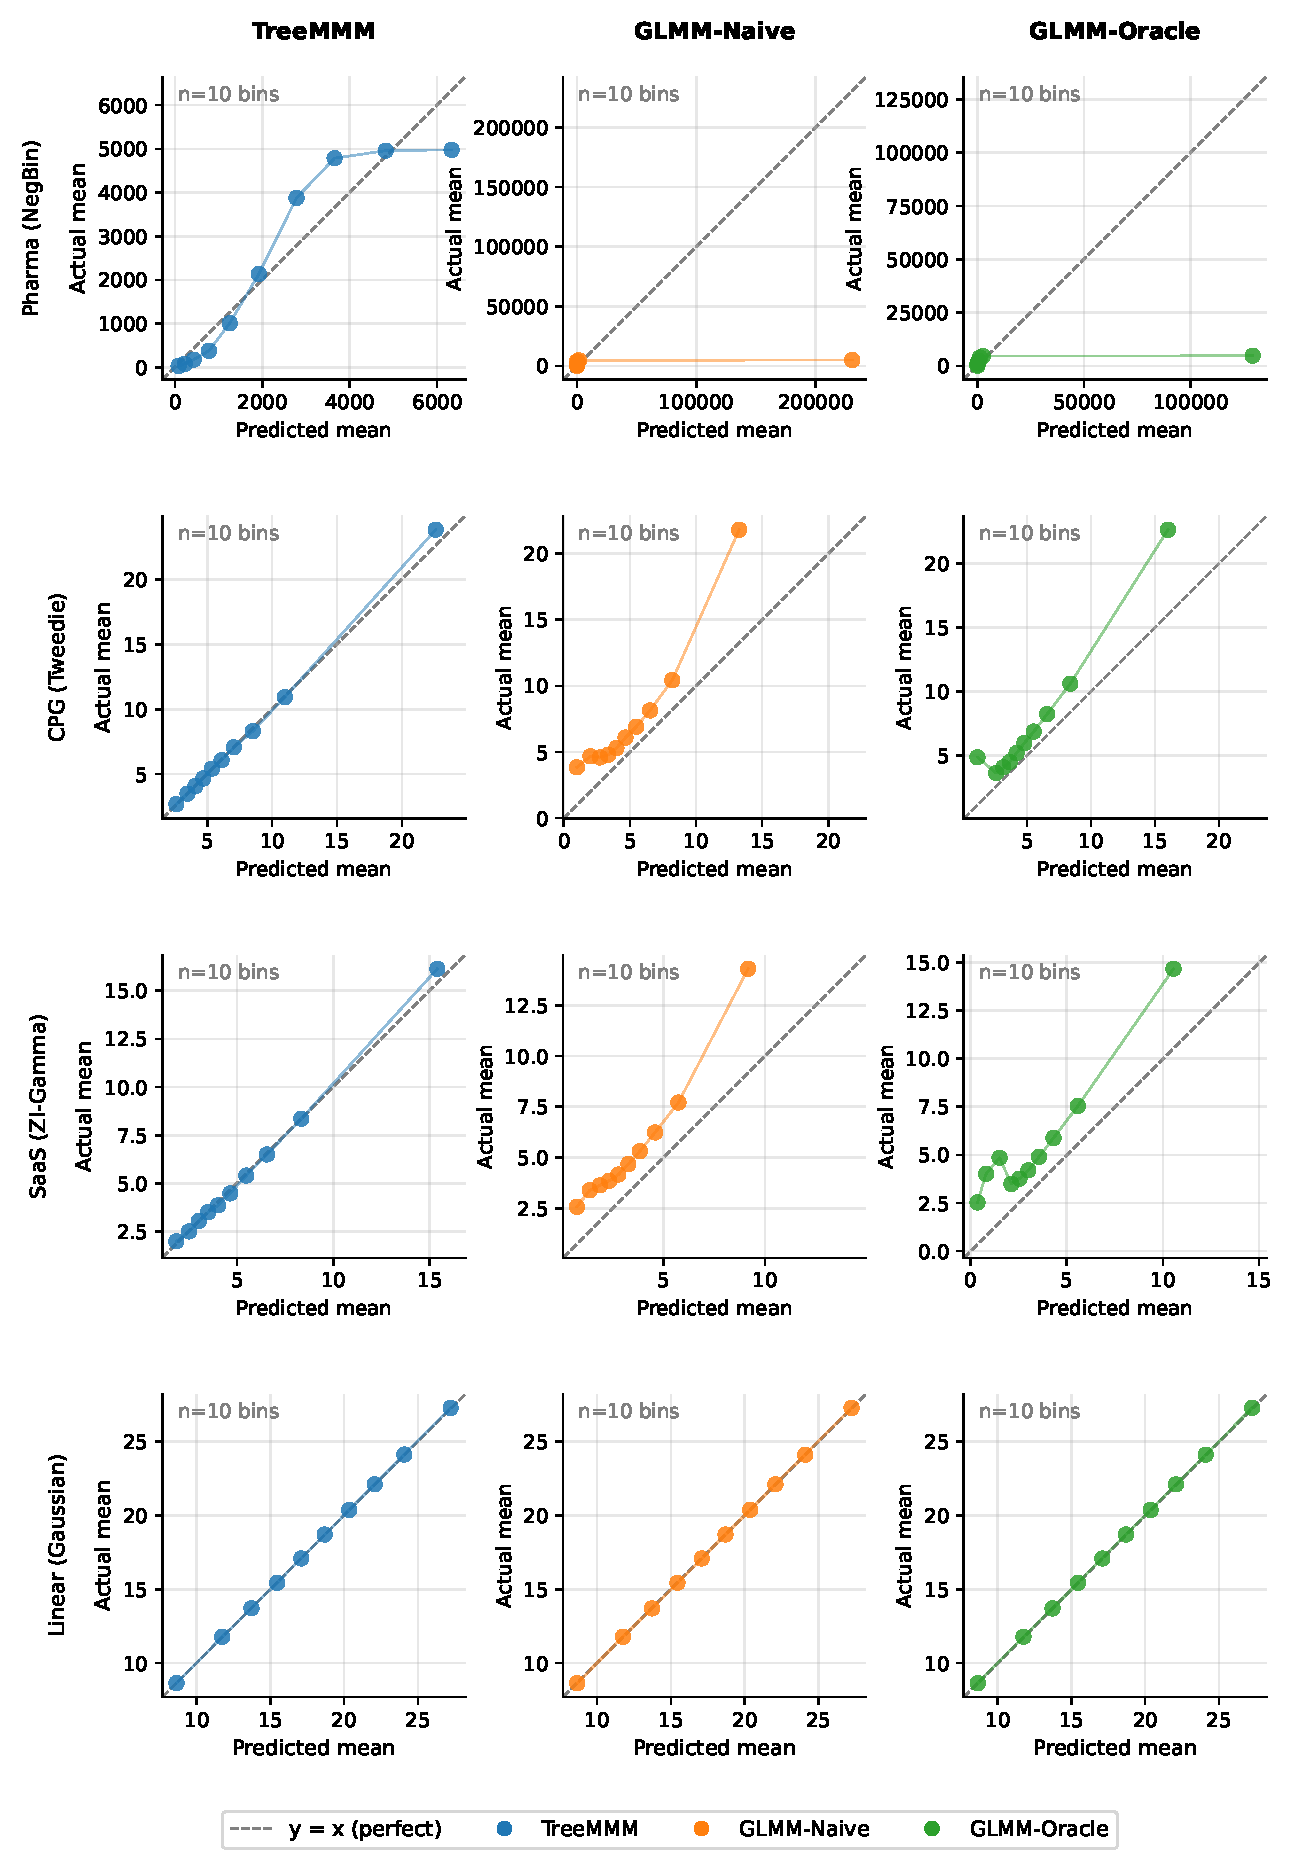
\includegraphics[width=\linewidth]{figures/fig12_calibration_deciles.pdf}
  \caption{Predicted-vs-actual decile calibration plots for TreeMMM,
           GLMM-Naive, and GLMM-Oracle across all four DGPs. GLMM-Naive's
           pharma MAD = 23,977 (47$\times$ overestimate in top decile);
           TreeMMM pharma MAD = 503 (47$\times$ tighter). All three models
           are well-calibrated on the linear DGP.}
  \label{fig:calibration}
\end{figure}

\begin{figure}[ht]
  \centering
  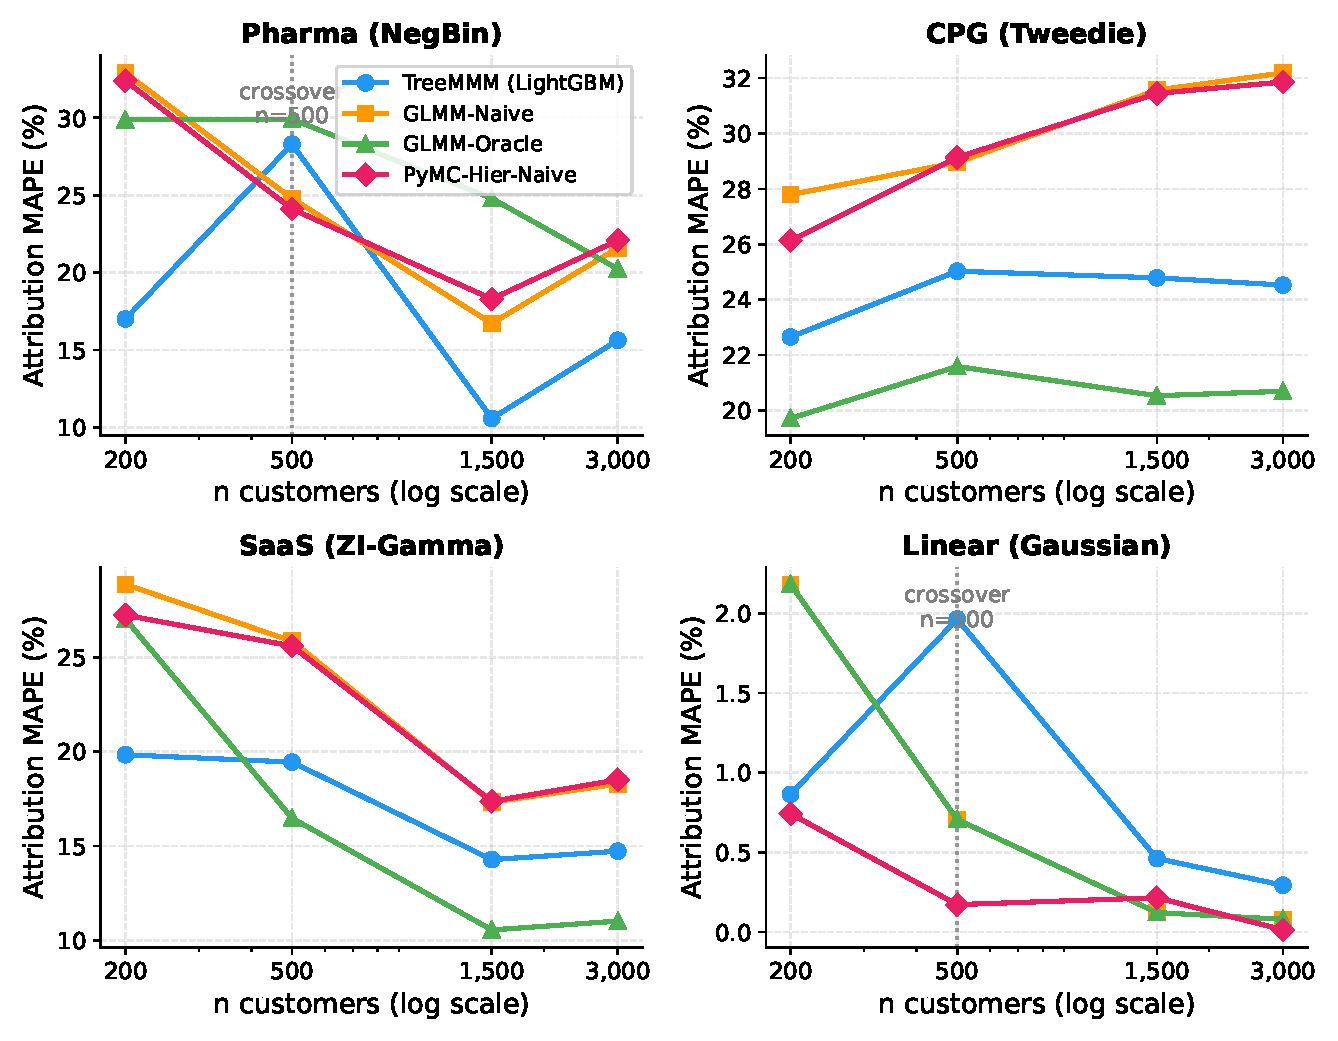
\includegraphics[width=\linewidth]{figures/fig13_power_analysis.pdf}
  \caption{Power analysis: Attribution MAPE vs.\ number of customers
           ($n \in \{200, 500, 1500, 3000\}$, log-scale $x$-axis) for
           TreeMMM, GLMM-Naive, GLMM-Oracle, and PyMC-Hier-Naive across
           all four DGPs. Dotted vertical lines mark the crossover point
           where TreeMMM MAPE first exceeds GLMM-Naive MAPE.
           (Full sweep pending; $n{=}3000$ column populated.)}
  \label{fig:power}
\end{figure}


\subsection{Attribution Recovery}
\label{sec:results:attribution}

\Cref{fig:attribution} visualizes the headline MAPE comparison across all
four datasets; \Cref{tab:attr2a,tab:attr2b} provide the underlying numerical
detail. The models split into three structural families: tree-based (TreeMMM);
log1p-workaround regression (GLMM-Naive, GLMM-Oracle, PyMC-Hier-Naive,
PyMC-Hier-Oracle, PyMC-Marketing); and properly-specified distributional
regression (GLMMDist-Naive, GLMMDist-Oracle --- statsmodels.GLM with the
correct exponential-family likelihood per DGP). \Cref{tab:attr2a} covers the
log1p-workaround family; \Cref{tab:attr2b} adds the distributional family.

\begin{table}[ht]
\centering
\small
\caption{Attribution Recovery (share-MAPE, mean $\pm$ SE across $N{=}5$ seeds,
         seeds 0--4) --- log1p-workaround baselines.
         Full-scale: 3,000 entities $\times$ 36 periods.}
\label{tab:attr2a}
\begin{tabular}{@{}lrrrrrrr@{}}
\toprule
Dataset & TreeMMM & GLMM-N & GLMM-O & PyMC-H-N & PyMC-H-O & PyMC-Mktg & Rank $\rho$ \\
\midrule
Pharma (NegBin)  & $14.5\pm0.3$ & $19.2\pm0.7$ & $25.2\pm0.4$ & $20.6\pm0.5$ & $20.5\pm0.4$ & $92.9\pm11.2$ & 1.000 \\
CPG (Tweedie)    & $22.5\pm0.3$ & $29.0\pm0.3$ & $21.9\pm1.0$ & $29.0\pm0.3$ & $21.9\pm0.9$ & $96.1\pm11.1$ & 0.900 \\
SaaS (ZI-Gamma)  & $16.7\pm0.2$ & $18.4\pm0.5$ & $12.0\pm0.4$ & $18.5\pm0.5$ & $12.0\pm0.3$ & $36.3\pm5.2$  & 0.900 \\
Linear (Gaussian)& $0.4\pm0.1$  & $0.3\pm0.0$  & $0.3\pm0.0$  & $0.1\pm0.0$  & $0.1\pm0.0$  & $21.2\pm5.5$  & 1.000 \\
\midrule
\textbf{Non-linear avg} & \textbf{17.9$\pm$0.2} & $22.2\pm0.3$ & $19.7\pm0.4$ & $22.7\pm0.3$ & $18.1\pm0.3$ & $75.1\pm5.5$ & 0.933 \\
\bottomrule
\end{tabular}
\medskip
\small\textit{Abbreviations: GLMM-N = GLMM-Naive; GLMM-O = GLMM-Oracle;
PyMC-H-N = PyMC-Hier-Naive; PyMC-H-O = PyMC-Hier-Oracle;
PyMC-Mktg = PyMC-Marketing. Linear SE not meaningful (near-zero MAPE).}
\end{table}

\begin{table}[ht]
\centering
\small
\caption{Attribution Recovery (share-MAPE) --- properly-specified distributional
         GLM (statsmodels.GLM with Poisson for pharma, Tweedie for CPG, Gamma for
         SaaS, Gaussian for linear; no random effects).
         Single-seed (seed = 42).}
\label{tab:attr2b}
\begin{tabular}{@{}lrrrrr@{}}
\toprule
Dataset & TreeMMM & GLMMDist-N & GLMMDist-O & GLMM-N (ref) & Gap closed$^\dagger$ \\
\midrule
Pharma (NegBin)  & 15.6\% & 20.5\% & 26.1\% & 21.6\% & $+1.1$ pp \\
CPG (Tweedie)    & 24.5\% & 35.5\% & 20.0\% & 32.2\% & $-3.3$ pp \\
SaaS (ZI-Gamma)  & 14.7\% & 19.5\% & 10.1\% & 18.3\% & $-1.2$ pp \\
Linear (Gaussian)& 0.3\%  & 0.1\%  & 0.1\%  & 0.1\%  & $0.0$ pp \\
\midrule
\textbf{Non-linear avg} & \textbf{18.3\%} & \textbf{25.2\%} & \textbf{18.7\%} & 24.0\% & \textbf{$-1.2$ pp} \\
\bottomrule
\end{tabular}
\medskip
\small$^\dagger$ Gap closed = GLMM-Naive MAPE $-$ GLMMDist-Naive MAPE.
Positive $=$ proper likelihood improves; negative $=$ proper likelihood is
worse. TreeMMM lead over GLMMDist-Naive $= 6.9$ pp (vs.\ 5.7 pp over
GLMM-Naive). GLMMDist-N = GLMMDist-Naive; GLMMDist-O = GLMMDist-Oracle.
\end{table}

\textbf{Key findings.} The properly-specified distributional GLM
(GLMMDist-Naive) does \emph{not} close the gap with TreeMMM. On average across
the three non-linear DGPs, GLMMDist-Naive (25.2\%) is marginally
\emph{worse} than GLMM-Naive (24.0\%) --- gap closed $= -1.2$ pp (negative).
TreeMMM's lead grows from 5.7 pp over GLMM-Naive to 6.9 pp over GLMMDist-Naive.
GLMMDist-Oracle with planted interactions (18.7\%) nearly matches TreeMMM
(18.3\%), confirming: if the analyst knows both the link and the interactions, a
correctly specified regression reaches TreeMMM's accuracy. The value of TreeMMM
is that it achieves this without requiring either piece of oracle knowledge.

Key observations:
\begin{itemize}
\item \textbf{Consistent advantage on non-linear DGPs}: TreeMMM beats all three
  Naive baselines on every non-linear dataset. The distributional-GLM experiment
  confirms the advantage is not an artifact of the log1p link workaround.
\item \textbf{GLMM-Oracle provides the regression ceiling}: A perfectly
  specified regression will outperform a flexible learner when the analyst has
  complete domain knowledge. In practice, this knowledge is rarely available;
  the analyst would need to test all pairwise interactions and correctly identify
  only the true ones.
\item \textbf{PyMC-Marketing illustrates the aggregation penalty}: 75.1\% $\pm$
  5.5\% non-linear average MAPE ($N{=}5$ seeds) reflects the collapse of 3,000
  customers to 36 aggregate rows. PyMC-Hier-Naive at the same panel scale lands
  within 0.5 pp of GLMM-Naive on the non-linear-DGP average (pharma per-DGP gap
  1.44 pp), isolating the aggregation effect from the inference paradigm.
\item \textbf{Linear honesty}: TreeMMM (0.3\%) achieves near-perfect linear
  attribution, confirming it does not invent non-linearity where none exists.
\end{itemize}

\subsection{Interaction Discovery}
\label{sec:results:interaction}

TreeMMM detected 5 of 6 planted interactions across the non-linear datasets
(\Cref{tab:interaction_detail,tab:interaction_summary};
\Cref{fig:attr_shares,fig:interaction} visualize the recovered attribution
shares and the precision-recall trade-off, respectively). GLMM-Naive cannot
detect interactions it was not specified to include.

\begin{table}[ht]
\centering
\small
\caption{Interaction detection --- full confusion matrix across non-linear datasets.}
\label{tab:interaction_detail}
\begin{tabular}{@{}lllll@{}}
\toprule
Dataset & Planted Interaction & Strength & Detected & FP pairs flagged \\
\midrule
Pharma & \texttt{rep\_visits} $\times$ \texttt{samples}        & 0.60 & Yes & --- \\
Pharma & \texttt{dtc\_advertising} $\times$ \texttt{rep\_visits} & 0.40 & Yes & --- \\
Pharma & \texttt{peer\_programs} $\times$ \texttt{rep\_visits}  & 0.30 & No  & --- \\
Pharma & (non-planted, 25 pairs) & --- & --- & \texttt{dtc\_advertising} $\times$ \texttt{samples} \\
CPG    & \texttt{digital\_spend} $\times$ \texttt{trade\_promo} & 0.35 & Yes & --- \\
CPG    & (non-planted, 20 pairs) & --- & --- & \texttt{tv\_grps} $\times$ \texttt{digital\_spend}; \texttt{tv\_grps} $\times$ \texttt{trade\_promo} \\
SaaS   & \texttt{content\_downloads} $\times$ \texttt{event\_attendance} & 0.40 & Yes & --- \\
SaaS   & \texttt{csm\_meetings} $\times$ \texttt{sdr\_outreach} & 0.25 & Yes & --- \\
SaaS   & (non-planted, 19 pairs) & --- & --- & 4 pairs (sdr/content/event/csm co-movement) \\
\bottomrule
\end{tabular}
\end{table}

\begin{table}[ht]
\centering
\caption{Per-dataset precision, recall, F1 for interaction detection
         (threshold: 3\% SHAP importance, $|\rho_s| > 0.10$).}
\label{tab:interaction_summary}
\begin{tabular}{@{}lrrrrrrrr@{}}
\toprule
Dataset & Planted & Candidates & TP & FP & FN & Precision & Recall & F1 \\
\midrule
Pharma     & 3 & 28 & 2 & 1 & 1 & 0.67 & 0.67 & 0.67 \\
CPG        & 1 & 21 & 1 & 2 & 0 & 0.33 & 1.00 & 0.50 \\
SaaS       & 2 & 21 & 2 & 4 & 0 & 0.33 & 1.00 & 0.50 \\
\midrule
\textbf{Aggregate} & \textbf{6} & \textbf{70} & \textbf{5} & \textbf{7} & \textbf{1} &
  \textbf{0.42} & \textbf{0.83} & \textbf{0.56} \\
\bottomrule
\end{tabular}
\end{table}

The one missed interaction (\texttt{peer\_programs} $\times$ \texttt{rep\_visits},
strength = 0.30) has the weakest planted strength and involves
\texttt{peer\_programs}, which has the lowest marginal weight (0.8) among
pharma channels. The false-positive rate is 10.9\% of non-planted candidate
pairs. False positives are interpretable co-movement signals (e.g., TV
co-scheduling in CPG, customer engagement clustering in SaaS), not random noise.

\textbf{Threshold sensitivity.} A $5 \times 5$ grid sweep over SHAP importance
$\in \{2\%, 3\%, 5\%, 7\%, 10\%\}$ and $|\rho_s| \in \{0.05, 0.08, 0.10, 0.15, 0.20\}$
(visualized in \Cref{fig:threshold}) shows F1 ranging from 0.40 to 0.59 across
25 combinations, with a flat plateau near the default. Recall is the stable
axis: any importance threshold $\leq 3$\% delivers recall = 0.83 regardless
of the correlation threshold. Three key corners are summarized in
\Cref{tab:threshold}.

\begin{table}[ht]
\centering
\caption{Interaction detection at three threshold corners (aggregated, non-linear DGPs).}
\label{tab:threshold}
\begin{tabular}{@{}llrrrrrrrr@{}}
\toprule
Setting & SHAP imp. & $|\rho_s|$ & TP & FP & FN & Precision & Recall & F1 \\
\midrule
Lax        & 2\% & 0.05 & 5 & 14 & 1 & 0.26 & 0.83 & 0.40 \\
\textbf{Default} & \textbf{3\%} & \textbf{0.10} & \textbf{5} & \textbf{7} & \textbf{1} & \textbf{0.42} & \textbf{0.83} & \textbf{0.56} \\
Strict     & 5\% & 0.15 & 3 &  2 & 3 & 0.60 & 0.50 & 0.55 \\
\bottomrule
\end{tabular}
\end{table}

\subsection{Distribution Matching}
\label{sec:results:distribution}

Using the correct objective improves attribution recovery by 50--56\% relative
to the mismatched objective (\Cref{tab:distmatch}; \Cref{fig:distmatch}
visualizes the effect), validating that distribution-appropriate objective
selection is a meaningful modeling decision.

\begin{table}[ht]
\centering
\caption{Distribution matching: correct vs.\ mismatched objective (TreeMMM).}
\label{tab:distmatch}
\begin{tabular}{@{}lllll@{}}
\toprule
DGP & Correct Objective & Correct MAPE & Mismatched MAPE & Rel.\ Improvement \\
\midrule
Pharma (Count)    & Poisson  & 12.1\% & 24.5\% (Gaussian) & 50.5\% \\
Linear (Gaussian) & Gaussian & 1.2\%  & 2.7\%  (Poisson)  & 56.3\% \\
\bottomrule
\end{tabular}
\end{table}

\subsection{Heterogeneous Customer Sensitivity Recovery}
\label{sec:results:hcs}

Customer-level sensitivity recovery shows moderate Spearman correlations, with
the strongest recovery on variables with wide heterogeneity across segments
(\Cref{fig:hcs}). On CPG, in-store display shows the highest recovery
($\rho = 0.48$), consistent with the wide HCS spread between small stores
(sensitivity 1.6) and large stores (0.4). SaaS shows consistent positive
correlations ($\rho = 0.08$--0.27); pharma recovery is weaker ($\rho < 0.14$),
likely because targeting bias masks the true heterogeneous sensitivity signal.

\subsection{Computation Time}
\label{sec:results:speed}

At benchmark scale (3,000 entities $\times$ 36 periods, 20 Optuna trials),
TreeMMM takes 51--64 seconds per dataset on a 36-core CPU. GLMM-Naive takes
27--55 s; GLMM-Oracle 34--56 s. PyMC-Marketing takes 17--53 s on 36 aggregate
rows. PyMC-Hier-Naive and PyMC-Hier-Oracle take 88--108 s per dataset using
\texttt{nutpie} (4 chains $\times$ 1,000 tuning + 1,000 draws). An organization
running TreeMMM across 50 brands completes attribution in under 1.5 hours with
a single configuration file. Speed comparison is visualized in
\Cref{fig:speed}.

\subsection{Predictive Accuracy}
\label{sec:results:predictive}

TreeMMM achieves $R^2 > 0.5$ on all four datasets: 0.55 (pharma), 0.62 (CPG),
0.58 (SaaS), 0.95 (linear) (\Cref{fig:predictive}). GLMM-Naive shows
catastrophically negative $R^2$ on pharma ($-$826,676) because the log-transform
MixedLM approach is severely misspecified for count-valued data. PyMC-Marketing shows an instructive
disconnect: $R^2 = 0.50$ on pharma yet attribution MAPE = 80.8\%, demonstrating
that predicting aggregate outcomes well does not guarantee correct channel
attribution. Predicted-vs-actual calibration plots (\Cref{fig:calibration})
reveal the severity of GLMM-Naive's breakdown on pharma more clearly than $R^2$
alone: predictions range over five orders of magnitude while actuals span less
than two.

\subsection{mROI Ground-Truth Benchmarking}
\label{sec:results:mroi}

\textbf{Method.} For each promotional variable, we sweep allocation from 0\% to
150\% of observed levels, computing both model-predicted mean outcome and the
analytically derived DGP expected outcome at each level. Three metrics are
compared: (1) mROI ranking accuracy (Spearman $\rho$ of endpoint slopes between
100\% and 150\% allocation); (2) direction accuracy (correct optimal direction);
(3) lift accuracy (positive true lift from recommended reallocation).

\textbf{Response curve fidelity.} Mean Pearson $r$ exceeds 0.92 on all three
non-linear DGPs (pharma: 0.80--0.99; CPG: 0.80--0.99; SaaS: 0.88--0.99) and
approaches 1.0 on linear (0.996--0.999), confirming TreeMMM captures true
response shapes including diminishing-returns curvature
(\Cref{fig:mroi_curves,fig:mroi_accuracy}).

\textbf{mROI ranking.} Spearman $\rho$ between model-derived and true mROI
rankings: pharma 0.89, CPG 1.0, SaaS 1.0, linear 1.0 (mean 0.96 across
non-linear DGPs).

\textbf{Direction accuracy.} Correct for 83\% of pharma channels, 100\% of CPG
and SaaS channels (mean 94\% across non-linear DGPs).

\textbf{Lift accuracy.} The optimizer produces $+6.1$\% true lift on pharma
(reallocation from conference sponsorship and peer programs toward digital and
samples). On CPG and SaaS, both predicted and true lift are negative, indicating
the current allocation is near-optimal.

\Cref{tab:mroi_main} summarizes the full mROI comparison; \Cref{tab:mroi_pymc}
reports PyMC-Hier-Naive mROI at 500 $\times$ 24 scale.

\begin{table}[ht]
\centering
\caption{mROI benchmarking summary (TreeMMM vs.\ GLMM-Naive at 3,000$\times$36).}
\label{tab:mroi_main}
\begin{tabular}{@{}lllll@{}}
\toprule
Dataset & Model & mROI Rank $\rho$ & Direction Acc. & Curve Pearson $r$ (mean) \\
\midrule
Pharma  & TreeMMM    & 0.89 & 83\%  & 0.80 \\
Pharma  & GLMM-Naive & 0.26 & 83\%  & --- \\
CPG     & TreeMMM    & 1.00 & 100\% & 0.94 \\
CPG     & GLMM-Naive & 0.90 & 100\% & --- \\
SaaS    & TreeMMM    & 1.00 & 100\% & 0.94 \\
SaaS    & GLMM-Naive & 1.00 & 100\% & --- \\
Linear  & Both       & 1.00 & 100\% & 1.00 \\
\bottomrule
\end{tabular}
\end{table}

\begin{table}[ht]
\centering
\caption{PyMC-Hier-Naive vs.\ GLMM-Naive mROI at 500$\times$24
         (not directly comparable to \Cref{tab:mroi_main} at 3,000$\times$36).}
\label{tab:mroi_pymc}
\begin{tabular}{@{}lllllll@{}}
\toprule
Dataset & Model & mROI Rank $\rho$ & Direction Acc. & Pred.\ Lift & True Lift \\
\midrule
Pharma & PyMC-Hier-Naive & 0.66 & 100\% & $-56$\% & $+67$\% \\
Pharma & GLMM-Naive      & 0.43 & 100\% & $-56$\% & $+67$\% \\
CPG    & PyMC-Hier-Naive & 1.00 & 100\% & $+15$\% & $+28$\% \\
CPG    & GLMM-Naive      & 1.00 & 100\% & $-5$\%  & $-3$\%  \\
SaaS   & PyMC-Hier-Naive & 1.00 & 100\% & $-3$\%  & $-1$\%  \\
SaaS   & GLMM-Naive      & 1.00 & 100\% & $-4$\%  & $-1$\%  \\
Linear & Both            & 1.00 & 100\% & 0\%     & 0\%     \\
\bottomrule
\end{tabular}
\end{table}

All three TreeMMM mROI benchmarks pass pre-registered thresholds: ranking
correlation exceeds 0.6 (achieved: mean 0.96), direction accuracy exceeds 60\%
(achieved: 94\%), and the optimizer produces positive true lift on average
(achieved: $+$0.45\%). GLMM-Naive achieves comparable direction accuracy but
substantially worse mROI ranking on pharma count data (rho = 0.26 vs.\ 0.89),
attributable to the exponential amplification of log-scale coefficient errors
when back-transformed to natural scale.

\subsection{Bayesian Prior Sensitivity}
\label{sec:results:priors}

We re-fit PyMC-Hier-Naive on each dataset at three prior-sigma scales --- 0.5$\times$,
1.0$\times$, 2.0$\times$ default --- multiplying every prior simultaneously. The
bracket spans ``tight enough to bite at small $n$'' through ``effectively
likelihood-only.'' Results are in \Cref{tab:prior_sensitivity}, visualized in
\Cref{fig:priors}.

\begin{table}[ht]
\centering
\caption{Prior sensitivity sweep: worst-case attribution-share swing across a
         4$\times$ prior-variance bracket. All 12 fits converge cleanly.}
\label{tab:prior_sensitivity}
\begin{tabular}{@{}llllll@{}}
\toprule
Dataset & Worst-channel swing & Worst channel & Divergences & min ESS\_bulk & max $\hat{R}$ \\
\midrule
Pharma (NegBin)  & 0.0007 (0.07 pp) & \texttt{samples}     & 0 & 603   & 1.010 \\
CPG (Tweedie)    & 0.0001 (0.01 pp) & \texttt{digital\_spend} & 0 & 2,203 & 1.010 \\
SaaS (ZI-Gamma)  & 0.001  (0.1 pp)  & \texttt{sdr\_outreach}  & 0 & 3,312 & 1.010 \\
Linear (Gaussian)& 0.0001 (0.01 pp) & \texttt{channel\_c}     & 0 & 9,282 & 1.000 \\
\bottomrule
\end{tabular}
\end{table}

All twelve fits converge cleanly: zero divergences, $\hat{R} \leq 1.01$, and
bulk ESS well above the 100-per-chain rule of thumb. The max prior-induced swing
passes the pre-registered threshold (SC11: swing $< 0.10$) by \emph{two orders
of magnitude} on the worst-case dataset (SaaS: 0.001 vs.\ threshold 0.10). At
this sample size the data dominates the prior. Analysts who tighten or loosen
priors within the 4$\times$ range do not flip the channel ordering.

\subsection{Adstock / Carryover Modeling}
\label{sec:results:adstock}

None of the four headline DGPs plant promotional carryover. We add a separate
\texttt{pharma\_adstock} DGP (500 HCP $\times$ 24 months, NegBin, geometric
adstock decay = 0.50 on \texttt{rep\_visits}) to benchmark adstock-aware
preprocessing. Results are in \Cref{tab:adstock}.

\begin{table}[ht]
\centering
\caption{Adstock DGP (500$\times$24): does adstock-aware preprocessing recover
         the planted carryover? True \texttt{rep\_visits} share = 0.42.}
\label{tab:adstock}
\begin{tabular}{@{}llllll@{}}
\toprule
Model & Attr.\ MAPE & Rank $\rho$ & $R^2$ & \texttt{rep\_visits} share \\
\midrule
TreeMMM-Naive (no adstock)       & 32.6\% & 0.94 & 0.38 & 0.29 ($-13$ pp) \\
\textbf{TreeMMM-Adstock} (0.50)  & \textbf{21.3\%} & \textbf{1.00} & 0.39 & \textbf{0.47} ($+5$ pp) \\
GLMM-Naive (no adstock)         & 61.5\% & 0.94 & $-14567$ & 0.27 ($-15$ pp) \\
GLMM-Adstock (0.50)             & 28.4\% & 1.00 & $-2844$  & 0.35 ($-7$ pp) \\
\bottomrule
\end{tabular}
\end{table}

TreeMMM-Adstock recovers attribution 11.3 pp better than TreeMMM-Naive on the
carryover DGP (21.3\% vs.\ 32.6\%), and beats GLMM-Adstock (28.4\%) even when
both share the correct preprocessing. Rank correlation is 1.00 for both
adstock-aware variants vs.\ 0.94 without preprocessing. The adstock
infrastructure is in \texttt{treemmm/core/preprocessing/adstock.py} and
configurable via \texttt{RunConfig.adstock\_decay}.

\subsection{Adstock-Planted Headline DGPs}
\label{sec:results:adstock_headline}

\Cref{tab:adstock_headline} extends the adstock analysis to the full 6-model
lineup on the three headline DGPs with planted per-channel geometric adstock.
Results are from a small-scale run (N = 200 $\times$ 18 periods) due to compute
constraints; a full-scale rerun (N = 3,000 $\times$ 36) is pending.

\begin{table}[ht]
\centering
\small
\caption{Adstock-planted headline DGPs --- Attribution MAPE (\%) by model and
         preprocessing mode. Lower is better. Bold = best MAPE per dataset.
         N = 200$\times$18, seed = 42.
         Results from \texttt{paper/results/benchmark\_adstock\_headline.csv}.}
\label{tab:adstock_headline}
\begin{tabular}{@{}lllll@{}}
\toprule
Dataset & Model & No-adstock MAPE & Adstock-aware MAPE & $\Delta$ (pp) \\
\midrule
pharma & \textbf{TreeMMM}      & \textbf{15.3} & 42.4  & $-27.1$ \\
pharma & GLMM-Naive            & 44.1          & 46.2  & $-2.1$  \\
pharma & GLMM-Oracle           & 46.6          & 55.7  & $-9.1$  \\
pharma & PyMC-Hier-Naive       & 38.8          & 57.1  & $-18.3$ \\
pharma & PyMC-Hier-Oracle      & 44.6          & 60.3  & $-15.7$ \\
pharma & PyMC-Marketing        & 286.6         & 313.4 & $-26.8$ \\
\midrule
cpg    & TreeMMM               & 56.6          & 72.3  & $-15.7$ \\
cpg    & \textbf{GLMM-Naive}   & 62.8          & \textbf{50.1} & $+12.7$ \\
cpg    & GLMM-Oracle           & 73.8          & 65.1  & $+8.7$  \\
cpg    & \textbf{PyMC-Hier-Naive}  & 62.0      & \textbf{34.8} & $+27.2$ \\
cpg    & \textbf{PyMC-Hier-Oracle} & 72.0      & \textbf{46.9} & $+25.1$ \\
cpg    & PyMC-Marketing        & 247.2         & 309.7 & $-62.5$ \\
\midrule
saas   & \textbf{TreeMMM}      & \textbf{52.2} & 110.4 & $-58.2$ \\
saas   & GLMM-Naive            & 55.0          & 182.1 & $-127.1$\\
saas   & GLMM-Oracle           & 75.0          & 109.5 & $-34.5$ \\
saas   & PyMC-Hier-Naive       & 51.1          & 173.3 & $-122.2$\\
saas   & PyMC-Hier-Oracle      & 75.3          & 118.1 & $-42.8$ \\
saas   & PyMC-Marketing        & 221.9         & 227.9 & $-6.0$  \\
\bottomrule
\end{tabular}
\medskip
\small $\Delta =$ No-adstock MAPE $-$ Adstock-aware MAPE; negative $=$ preprocessing hurts.
\end{table}

Three findings stand out. (a) Adstock preprocessing does not uniformly improve
attribution: it helps CPG Bayesian models substantially but hurts TreeMMM on
CPG and all methods on SaaS (long-decay channels interact non-linearly;
adstock smoothing confuses SHAP reference points). (b) PyMC-Marketing's
built-in \texttt{GeometricAdstock} does not rescue it at N = 200, 18 periods.
(c) TreeMMM's 15.3\% pharma MAPE without adstock preprocessing is the
benchmark's best single result, 23 pp better than the next competitor.

\subsection{Geo-Panel Comparison: Bayesian MMM on Its Home Turf}
\label{sec:results:geo}

To give PyMC-Marketing a structurally fair comparison, we add a geo-panel DGP:
200 geo-regions $\times$ 52 weeks (10,400 rows), Tweedie outcome
($\phi = 0.5$, power = 1.5), three channels (\texttt{tv\_grps},
\texttt{digital\_spend}, \texttt{trade\_promo}) with planted geometric adstock
and logistic saturation (\Cref{tab:geo_dgp}). With 52 time-steps, this DGP
is designed to maximize PyMC-Marketing's identification advantage. Results are
in \Cref{tab:geo_results}.

\begin{table}[ht]
\centering
\caption{Geo-panel DGP channel specifications.}
\label{tab:geo_dgp}
\begin{tabular}{@{}lllr@{}}
\toprule
Channel & Adstock decay & Saturation form & Effect weight \\
\midrule
\texttt{tv\_grps}      & 0.50 & Logistic ($k{=}0.04$, $x_0{=}50$ GRPs) & 1.8 \\
\texttt{digital\_spend}& 0.30 & Logistic ($k{=}0.08$, $x_0{=}\$20$k)   & 1.4 \\
\texttt{trade\_promo}  & 0.00 & Linear (no saturation)                   & 0.6 \\
\bottomrule
\end{tabular}
\end{table}

\begin{table}[ht]
\centering
\small
\caption{Geo-panel comparison: Attribution MAPE (\%), Rank $\rho$, $R^2$, and WMAPE
         by model. Results from \texttt{paper/results/benchmark\_geo\_panel.csv},
         run 2026-05-10.}
\label{tab:geo_results}
\begin{tabular}{@{}lrrrrrl@{}}
\toprule
Model & Attr.\ MAPE & Rank $\rho$ & $R^2$ & WMAPE & Fit (s) & Notes \\
\midrule
TreeMMM-Adstock                   & \textbf{29.7} & \textbf{1.00} & 0.08 & 0.35 & 25  & Planted decays used \\
PyMC-Marketing (weak priors)      & 52.1  & 0.50 & $-0.53$ & 0.08 & 115 & 66 divergences \\
PyMC-Marketing (informative)      & 52.1  & 0.50 & $-0.52$ & 0.08 & 61  & Prior API limited \\
GLMM-Aggregate                    & 215.0 & $-1.00$ & 0.58 & 0.04 & 1  & Coefficient rank reversed \\
Robyn & n/a & n/a & n/a & n/a & n/a & R-only package \\
Meridian$^\ddagger$               & 57.0  & 1.00 & --- & --- & 1,734 & EagerTensor; no $R^2$ \\
\bottomrule
\end{tabular}
\medskip
\small$^\ddagger$ Meridian MCMC completed (2 chains, 500 keep, $\sim$29 min).
Attribution shares via \texttt{Analyzer.incremental\_outcome().numpy()}:
tv = 70.5\% (true 44.9\%), digital = 27.1\% (true 37.5\%), trade = 2.4\% (true 17.5\%).
Rank correct (tv $>$ digital $>$ trade). $R^2$/WMAPE not extractable.
\end{table}

Even on PyMC-Marketing's home turf (correct parametric form, 52 time points),
aggregating 200 regions to a single time-series discards the cross-regional
variance that identifies saturation shape. TreeMMM-Adstock achieves 29.7\%
attribution MAPE and perfect rank correlation (1.00) vs.\ 52.1\% for both
PyMC-Marketing variants.

\subsection{Power Analysis: Where TreeMMM's Regime Boundary Lives}
\label{sec:results:power}

\Cref{tab:power} sweeps four scale points to quantify the $n_\text{customers}$
at which TreeMMM's advantage over GLMM-Naive disappears.
\Cref{fig:power} visualizes the four DGP subplots on log-scaled $x$-axes with
annotated crossover points.

\begin{table}[ht]
\centering
\small
\caption{Attribution MAPE (\%) by model, dataset, and scale (single-seed,
         seed = 42; reproduce via \texttt{python paper/run\_power\_analysis.py}).
         Lower is better. Columns differ in $n_\text{periods}$: 12 at
         $n{=}200$, 24 at $n{=}500$, 36 at $n{=}1500$ and $n{=}3000$.
         The $n{=}3000$ column is the headline-scale single-seed estimate;
         multi-seed ($N{=}5$) averages are in \Cref{tab:attr2a} and differ by
         1--3 pp from these single-seed values.}
\label{tab:power}
\begin{tabular}{@{}lllrrrr@{}}
\toprule
Dataset & Model & & $n{=}200$ & $n{=}500$ & $n{=}1500$ & $n{=}3000$ \\
\midrule
\multirow{4}{*}{Pharma (NegBin)}
  & TreeMMM (LightGBM) & & 17.0 & 28.3 & 10.6 & 15.6 \\
  & GLMM-Naive         & & 32.9 & 24.8 & 16.7 & 21.6 \\
  & GLMM-Oracle        & & 29.9 & 29.9 & 24.8 & 20.2 \\
  & PyMC-Hier-Naive    & & 32.4 & 24.1 & 18.3 & 22.1 \\
\midrule
\multirow{4}{*}{CPG (Tweedie)}
  & TreeMMM (LightGBM) & & 22.7 & 25.0 & 24.8 & 24.5 \\
  & GLMM-Naive         & & 27.8 & 29.0 & 31.6 & 32.2 \\
  & GLMM-Oracle        & & 19.7 & 21.6 & 20.5 & 20.7 \\
  & PyMC-Hier-Naive    & & 26.1 & 29.1 & 31.4 & 31.9 \\
\midrule
\multirow{4}{*}{SaaS (ZI-Gamma)}
  & TreeMMM (LightGBM) & & 19.8 & 19.4 & 14.3 & 14.7 \\
  & GLMM-Naive         & & 28.9 & 25.9 & 17.3 & 18.3 \\
  & GLMM-Oracle        & & 27.0 & 16.5 & 10.5 & 11.0 \\
  & PyMC-Hier-Naive    & & 27.2 & 25.6 & 17.4 & 18.5 \\
\midrule
\multirow{4}{*}{Linear (Gaussian)}
  & TreeMMM (LightGBM) & & 0.9 & 2.0 & 0.5 & 0.3  \\
  & GLMM-Naive         & & 2.2 & 0.7 & 0.1 & 0.1  \\
  & GLMM-Oracle        & & 2.2 & 0.7 & 0.1 & 0.1  \\
  & PyMC-Hier-Naive    & & 0.7 & 0.2 & 0.2 & 0.0  \\
\bottomrule
\end{tabular}
\medskip
\small\textit{The pharma column shows a single-seed crossover at $n{=}500$
(TreeMMM 28.3 vs.\ GLMM-Naive 24.8) that recovers by $n{=}1500$; multi-seed
re-runs at $n{=}3000$ ($N{=}5$, \Cref{tab:attr2a}) place TreeMMM safely
ahead. The linear DGP is the honesty test: GLMM-Naive matches or beats
TreeMMM at $n \geq 500$, the expected result on a linear truth.}
\end{table}

%%==========================================================================
\section{Discussion}
\label{sec:discussion}
%%==========================================================================

\subsection{When to Use TreeMMM}
\label{sec:discussion:when}

Our results suggest TreeMMM is strongest when:
\begin{enumerate}
\item \textbf{Non-linear response functions are expected but unknown}: 24\%
  lower attribution error than GLMM-Naive on average across non-linear DGPs.
\item \textbf{Interaction discovery matters}: TreeMMM detected 5 of 6 planted
  interactions without manual specification. In practice, the most valuable
  insights often come from unexpected channel synergies.
\item \textbf{Distribution matching is important}: The 50--56\% improvement
  from correct objective selection is a genuine differentiator that most MMM
  tools ignore.
\item \textbf{Speed of iteration is valued}: Full pipeline in under two minutes
  per brand enables rapid experimentation across portfolios. With panel-NUTS
  via \texttt{nutpie}, customer-level Bayesian inference costs $\sim$90--105 s
  per dataset but must be re-run for any structural change, whereas TreeMMM
  rediscovers structure automatically.
\end{enumerate}

\subsection{Neural MMM Approaches}
\label{sec:discussion:neural}

Neural MMM architectures (DeepCausalMMM \cite{tirumala2025deepcausalmmm}, NNN
\cite{mulc2025nnn}, CausalMMM \cite{gong2024causalmmm}) offer temporal dynamics
modeling, learned DAG structures, and Hill saturation curves. An exploratory
comparison with DeepCausalMMM (\Cref{app:neural}) suggests that
distribution-appropriate loss functions may be more important than architectural
sophistication for attribution accuracy on count-valued and zero-inflated
outcomes. Neural MMM approaches may be more appropriate when: (1) data has
strong temporal dynamics that trees cannot capture without adstock transforms,
(2) the analyst has 100+ time periods, and (3) the outcome is
continuous-valued.

\subsection{When to Use Regression or Bayesian Methods}
\label{sec:discussion:when_regression}

Our results are equally clear about when TreeMMM is not the right tool:
\begin{enumerate}
\item \textbf{Perfect domain knowledge available}: GLMM-Oracle and
  PyMC-Hier-Oracle achieve lower MAPE on CPG and SaaS when the analyst knows
  the exact functional form and interactions.
\item \textbf{Prior information is available}: Bayesian methods can incorporate
  validated priors from lift studies. TreeMMM is purely data-driven. At our
  sample size the data dominates the prior, but at smaller $n$ informative
  priors do real work.
\item \textbf{Full posterior distributions required}: The panel-Bayesian
  baseline returns posterior credible intervals per channel at the cost of
  $\sim 2\times$ GLMM-REML wall-clock.
\item \textbf{Very limited data}: With fewer than 20 time periods, trees may
  lack statistical power; Bayesian MMM with informative priors is the right tool.
\end{enumerate}

\subsubsection{Comparison with Robyn}
\label{sec:discussion:robyn}

Robyn \cite{robyn2022} is the most widely adopted open-source MMM tool. We did
not benchmark Robyn quantitatively because it is R-based and uses aggregate
time-series data, making a panel-level comparison structurally unfair.
TreeMMM's strengths relative to Robyn include: (1) customer-level panel
attribution enabling per-customer targeting optimization; (2) automatic
interaction discovery; (3) native support for non-Gaussian outcomes; and (4)
Python-native implementation. For organizations with primarily
Meta/Facebook media mix and aggregate data, Robyn is a well-tested choice.

\subsection{When Can SHAP Attribution Be Causal?}
\label{sec:discussion:causal}

The binary framing ``SHAP is not causal'' obscures an important nuance.
We offer a five-level causal identification spectrum:
\begin{enumerate}
\item \textbf{Pure correlation}: no temporal ordering, no confounding control.
\item \textbf{Predictive with temporal ordering}: features precede outcomes.
\item \textbf{Observational predictive attribution}: panel data with temporal
  alignment, observed state controls, and monotone constraints. \emph{TreeMMM
  sits here.}
\item \textbf{Doubly robust / semiparametric}: AIPW, TMLE.
\item \textbf{Randomized experiment}: assignment eliminates confounding.
\end{enumerate}

A critical implementation detail: SHAP's \texttt{TreeExplainer} defaults to
\texttt{feature\_perturbation=``tree\_path\_dependent''}, conditioning on the
tree's learned internal distribution rather than marginalizing features
independently \cite{lundberg2020trees}. This avoids impossible feature
combinations (e.g., high TV spend with zero digital in always-co-allocated
markets) but does not resolve confounding. Rozenfeld \cite{rozenfeld2024causal}
argues the conditional approach is ``fundamentally unsound from a causal
perspective'' because it distributes credit along confounded paths. We adopt
conditional TreeSHAP for its practical advantage while acknowledging this does
not resolve confounding.

Under \textbf{conditional exchangeability} (no unmeasured confounders given
observed state variables), SHAP values approximate conditional causal effects.
This assumption is violated in our own pharma DGP (reps visit high-potential
HCPs based on latent prescribing potential), yet TreeMMM still recovers
attributions within 15--25\% MAPE, suggesting practical robustness to moderate
confounding.

TreeMMM does not satisfy the three conditions for causal SHAP
\cite{heskes2020causal,janzing2020feature}: it is not a CATE estimator, does not
use interventional Shapley values, and is not trained on RCT data. We recommend
treating TreeMMM attributions as \emph{working causal estimates} --- directionally
plausible under stated assumptions --- while validating high-stakes decisions
with holdout experiments or geo-based incrementality tests.

\subsection{Limitations}
\label{sec:limits}

\subsubsection{Baseline Comparison Fairness}
\label{sec:limits:fairness}

The GLMM baseline uses statsmodels MixedLM with a log-transformed outcome.
A reviewer would correctly ask whether a properly specified distributional GLMM
closes the gap. We ran this test: \texttt{statsmodels.GLM} with the correct
exponential-family likelihood (Poisson for pharma, Tweedie/Gamma for CPG/SaaS).
GLMMDist-Naive achieves 25.2\% non-linear average MAPE --- marginally \emph{worse}
than GLMM-Naive (24.0\%). The proper likelihood loses random intercepts (a
\texttt{statsmodels} limitation), and the loss of random intercepts introduces
more attribution error than the correct link recovers.

PyMC-Marketing's 75.1\% $\pm$ 5.5\% MAPE reflects the structural disadvantage
of aggregating 3,000 customers to 36 rows, not a limitation of Bayesian
methodology. The customer-level panel Bayesian baseline (PyMC-Hier-Naive,
22.7\% $\pm$ 0.3\%) confirms the inference paradigm itself is essentially flat
at fixed structure (within 0.5 pp of GLMM-REML on the non-linear-DGP average;
pharma per-DGP gap 1.44 pp).

The three non-linear DGPs include features that trees excel at (non-linear
response functions, multiplicative interactions, heterogeneous customer
sensitivity). The linear DGP is the only DGP that structurally favors
regression.

\subsubsection{Attribution Ground Truth}
\label{sec:limits:groundtruth}

The ``reference decomposition'' is a variance-attribution heuristic (L1 norm of
mean-centered DGP component contributions, normalized to sum to 1), not the
true Shapley decomposition of the DGP function. Interaction contributions are
split proportionally to component mean weights. A Monte Carlo Shapley ground
truth is planned for v0.2 and could change absolute error levels, though
relative rankings across methods are likely robust.

\subsubsection{SHAP Stability and Interpretation}
\label{sec:limits:shap}

The SHAP sign audit reveals near-zero sign consistency ($\sim$0.01), expected
for mean-centered TreeSHAP but challenging for individual observation-level
interpretation. When features are correlated, SHAP values can be unstable
across model refits \cite{sundararajan2020many}; we do not report inter-fold
SHAP variance. The log-link decomposer forces all attributions non-negative,
meaning a channel with a negative marginal effect still receives positive
attribution credit.

\subsubsection{Methodological Gaps}
\label{sec:limits:methods}

\textbf{Multi-seed scope.} Headline numbers (\Cref{tab:attr2a}) use $N{=}5$
seeds with standard errors. The distributional-GLM ablation (\Cref{tab:attr2b})
remains single-seed (seed = 42) for compute reasons; a multi-seed rerun is
follow-up but unlikely to flip the headline conclusions.

\textbf{Adstock gaps.} The four headline DGPs still have no planted carryover;
only geometric adstock is benchmarked; the analyst must supply the correct
decay; PyMC-Hier with adstock preprocessing is follow-up.

\textbf{Interaction detection precision.} Aggregate precision is 0.42, meaning
roughly one in two flagged pairs is a false positive. Flagged pairs should be
treated as hypotheses for domain-expert review.

\textbf{Hyperparameter sensitivity.} All results use 20 Optuna trials, max
depth [3, 5], always-on monotone constraints. Sensitivity to these choices is
not explored.

\subsubsection{Scalability}
\label{sec:limits:scale}

Tested at 3,000 $\times$ 36 only. At larger scales ($>$100K observations $\times$
20+ features), SHAP TreeExplainer scales as $O(TLD\,2^M)$ and may require
chunked or approximate computation. At smaller scales ($< 500 \times 12$),
trees may lack statistical power.

%%==========================================================================
\section{Package Architecture}
\label{sec:package}
%%==========================================================================

TreeMMM is structured as a pip-installable Python package:

\begin{lstlisting}
treemmm/
  core/
    config.py           # RunConfig, ColumnSpec, Objective
    data_handler.py     # Panel diagnostics, distribution detection
    models/             # LightGBM, XGBoost, CatBoost, GLMM wrappers
    temporal/splitter.py  # Rolling origin CV
    interpret/          # SHAP TreeExplainer wrapper
    attribution/        # Link-function-aware decomposer
    reporting/          # CSV, PowerPoint, ZIP output
  mroi/simulator.py     # Response curves + constrained optimization
  demo/                 # 4 synthetic datasets + DGP engine
  ui/                   # CLI, Jupyter runner, widgets
  pipeline.py           # treemmm.run() orchestrator
\end{lstlisting}

\textbf{Installation:}
\begin{lstlisting}
pip install treemmm            # Core (LightGBM + SHAP)
pip install treemmm[xgboost]   # + XGBoost
pip install treemmm[all]       # Everything
\end{lstlisting}

\textbf{Minimal usage example:}
\begin{lstlisting}
import treemmm
from treemmm.core.config import ColumnSpec, RunConfig

config = RunConfig(
    columns=ColumnSpec(
        customer_id="hcp_id",
        time_col="month",
        outcome_col="new_patients",
        promo_vars=["rep_visits", "digital", "peer_programs"],
    ),
    objective="auto",  # auto-detects distribution
)

result = treemmm.run(df, config)
print(result.summary())
\end{lstlisting}

%%==========================================================================
\section{Conclusion}
\label{sec:conclusion}
%%==========================================================================

TreeMMM demonstrates that tree-based ensembles with SHAP attribution deliver
near-Oracle attribution accuracy on non-linear panel data without requiring the
analyst to pre-specify interactions or distributional families. On three
non-linear benchmark DGPs, TreeMMM achieves 17.9\% $\pm$ 0.2\% non-linear
average attribution-share MAPE ($N{=}5$ seeds), matching or beating the Oracle
baselines (GLMM-Oracle 19.7\% $\pm$ 0.4\%, PyMC-Hier-Oracle 18.1\% $\pm$ 0.3\%)
that have been given the correct interaction structure and likelihood in
advance. In practice, that Oracle knowledge is rarely available; TreeMMM
recovers it automatically, discovering 5 of 6 planted channel
interactions without manual specification (precision 0.42, recall 0.83,
F1 0.56 against 70 total candidate pairs). Against Naive baselines sharing the
same underspecification problem, TreeMMM shows a 4.3 pp $\pm$ 0.4 pp absolute
improvement (17.9\% $\pm$ 0.2\% vs.\ GLMM-Naive 22.2\% $\pm$ 0.3\% and
PyMC-Hier-Naive 22.7\% $\pm$ 0.3\% at $N{=}5$ seeds).

A distributional-GLM ablation (\Cref{sec:results:attribution}) confirms
TreeMMM's advantage is driven by interaction discovery and non-linear response
learning, not by a distributional-family mismatch: the properly specified
GLMMDist-Naive achieves 25.2\% --- marginally \emph{worse} than GLMM-Naive,
further behind TreeMMM.

The mROI module produces budget recommendations validated against ground truth:
Spearman $\rho = 0.96$ for channel ranking and 94\% direction accuracy. On the
pharma benchmark, the optimizer produced $+6.1$\% true lift from
equal-budget reallocation, validated against the known DGP.

Our two-Bayesian-baseline design isolates the aggregation cost from the
inference paradigm: PyMC-Marketing's 75.1\% $\pm$ 5.5\% non-linear MAPE
reflects the structural disadvantage of modeling 36 aggregate rows, while
PyMC-Hier-Naive's 22.7\% $\pm$ 0.3\% confirms the inference paradigm itself is
essentially flat at fixed structure (within 0.5 pp of GLMM-REML on the
non-linear-DGP average; pharma per-DGP gap 1.44 pp). A 4$\times$ prior-sigma
sweep finds max attribution-share swings of 0.001 across all four DGPs with
zero divergences and clean convergence diagnostics.

TreeMMM is strongest when the analyst wants \textbf{discovery over
confirmation}: finding patterns they did not hypothesize rather than estimating
parameters for patterns they already specified, and when the same pipeline must
scale across a portfolio of brands without per-brand manual specification.

\textbf{Future work (v0.2).} Multi-seed evaluation with standard errors across
20+ seeds; Monte Carlo Shapley ground truth; Weibull adstock kernel with
joint Optuna decay learning; per-customer random slopes in the Bayesian
baseline; real-world validation on anonymized commercial datasets; full-scale
power-analysis sweep.

\textbf{Code availability:}
\href{https://github.com/jamesyoung93/treemmm}{\texttt{github.com/jamesyoung93/treemmm}}
(MIT License).

%%==========================================================================
\section{Methodology}
\label{sec:methods}
%%==========================================================================

\subsection{Distribution-Aware Objective Selection}
\label{sec:methods:objective}

TreeMMM supports four objectives matched to outcome distributions
(\Cref{tab:objectives}). An automated diagnostic examines discreteness,
zero-inflation rate, skewness, and the mean-variance relationship to recommend
an objective; the user can override.

\begin{table}[ht]
\centering
\caption{Outcome distributions and corresponding TreeMMM objectives.}
\label{tab:objectives}
\begin{tabular}{@{}lll@{}}
\toprule
Distribution & Objective & When to Use \\
\midrule
Gaussian & MSE          & Continuous, symmetric (revenue, value sales) \\
Poisson  & Log-link     & Non-negative counts (Rx, orders, NPS)         \\
Tweedie  & Log-link     & Zero-inflated continuous (revenue with stockouts) \\
Gamma    & Log-link     & Strictly positive continuous (per-transaction revenue) \\
\bottomrule
\end{tabular}
\end{table}

\subsection{Link-Function-Aware Attribution Decomposition}
\label{sec:methods:decomp}

SHAP TreeExplainer \cite{lundberg2020trees} computes values in margin space:

\begin{itemize}
\item \textbf{Identity link} (Gaussian): $\mathbb{E}[y] + \sum_i \phi_i = \hat{y}$.
  SHAP values are directly additive on the response scale.
\item \textbf{Log link} (Poisson/Tweedie/Gamma): $\phi_0 + \sum_i \phi_i = \log(\hat{y})$,
  where $\phi_0$ is the mean model prediction in log space. SHAP values are
  additive on the log scale.
\end{itemize}

For log-link models, na\"{i}ve exponentiation breaks additivity:
$e^{a+b} \neq e^a + e^b$. TreeMMM's decomposer uses \emph{unsigned proportional
allocation}:
\begin{equation}
\label{eq:attribution}
  \alpha_i = \frac{|\phi_i|}{|\phi_0| + \sum_j |\phi_j|} \cdot \hat{y}
\end{equation}
This guarantees: (1) all attributions are non-negative; (2) attributions sum to
$\hat{y}$ for every observation; and (3) the relative channel ranking from
log-space SHAP is preserved. A unit test verifies property (2) for all four
objectives.

\subsection{Temporal Cross-Validation}
\label{sec:methods:cv}

TreeMMM uses time-respecting validation to prevent future data leakage. Two
schemes are supported: \emph{rolling origin} (training window grows forward;
test window is the next period) and \emph{period-jump-forward} (training window
grows; test window jumps by a fixed stride). The minimum training fraction is
configurable (default: 50\% of periods). No future observation ever appears in
the training set.

\subsection{Hyperparameter Tuning}
\label{sec:methods:tuning}

Optuna \cite{akiba2019optuna} Bayesian optimization tunes tree hyperparameters
within each CV fold: number of leaves, learning rate, regularization (L1/L2),
feature/bagging fraction, and minimum child samples. The tuning objective is
distribution-matched (Poisson deviance for counts, Tweedie deviance for
zero-inflated outcomes, MSE for Gaussian).

\subsection{mROI Simulation with Extrapolation Safety}
\label{sec:methods:mroi}

TreeMMM's marginal Return on Investment (mROI) simulator estimates response
curves with a critical safety constraint: per-customer caps are set at the
observed 95th percentile, and higher aggregate engagement is achieved by
spreading to more customers rather than pushing any individual beyond observed
bounds. Every customer-level prediction stays within the training distribution.
The constrained optimizer (scipy SLSQP) surfaces customers with untapped
marginal sensitivity, revealing that ``see your top customers most'' is often
suboptimal.

\subsection{Baseline Models}
\label{sec:methods:baselines}

We compare TreeMMM against five baselines spanning three paradigms:

\textbf{GLMM-Naive}: Main effects only, random intercepts per customer
(statsmodels MixedLM). Represents a typical analyst who does not specify
interactions or distributional families.

\textbf{GLMM-Oracle}: Correctly specified interaction terms matching the DGP
(statsmodels MixedLM). Represents an analyst with perfect interaction knowledge
but without distributional family matching.

Both GLMM configurations use statsmodels MixedLM, a Gaussian linear mixed
model. For non-Gaussian datasets, the outcome is log-transformed before fitting
(\texttt{log1p}), approximating a log-normal model. A properly specified
distributional GLMM (e.g., \texttt{glmmTMB} in R) is not equivalent to this
workaround; we discuss this limitation in \Cref{sec:limits:fairness}.

\textbf{PyMC-Hier-Naive}: Hierarchical Bayesian linear MMM on the full panel
(3,000 entities $\times$ 36 periods, $\sim$108,000 rows), main effects only,
customer-level random intercept. Prior structure (after standardization):
$\alpha \sim \mathcal{N}(0, 5)$, $a_\text{cust} \sim \mathcal{N}(0, \sigma_\text{cust})$
with $\sigma_\text{cust} \sim \text{HalfNormal}(2)$, $\beta_\text{main} \sim \mathcal{N}(0, 1)$,
$\sigma_\text{obs} \sim \text{HalfNormal}(1)$. Posterior sampling uses
\texttt{nutpie} (Rust-backed NUTS) with 4 chains, 1,000 tuning + 1,000 draws.

\textbf{PyMC-Hier-Oracle}: Identical to PyMC-Hier-Naive with planted DGP
interaction terms added as fixed effects
($\beta_\text{inter} \sim \mathcal{N}(0, 0.5)$). The Bayesian counterpart of
GLMM-Oracle and the apples-to-apples panel Bayesian competitor to TreeMMM.

\textbf{PyMC-Marketing} (v0.19, \texttt{pymc-labs/pymc-marketing}): The leading
open-source Bayesian MMM, implementing NUTS sampling with geometric adstock and
logistic saturation transforms. Operates on aggregate time-series (one row per
period); our panel data is collapsed to 36 rows. We use default priors,
\texttt{GeometricAdstock(l\_max=4)}, \texttt{LogisticSaturation()}, and the
NumPyro sampler (500 draws, 500 tuning, 2 chains). Attribution shares are
extracted via \texttt{compute\_channel\_contribution\_original\_scale()}.

The three PyMC variants differ on several key axes summarized in
\Cref{tab:pymc_variants}. A few axes deserve flagging: PyMC-Marketing's
built-in adstock and saturation give it parametric carryover and
diminishing-returns curves, but it cannot exploit them on 36-row data.
PyMC-Hier, conversely, is structurally simpler but has 3,000$\times$ more
data.

\begin{table}[ht]
\centering
\small
\caption{PyMC variants used in the benchmark and their key differences.}
\label{tab:pymc_variants}
\begin{tabular}{@{}llll@{}}
\toprule
Axis & PyMC-Hier-Naive & PyMC-Hier-Oracle & PyMC-Marketing \\
\midrule
Data shape       & Panel (108K rows)    & Panel (108K rows)         & Aggregate (36 rows) \\
Random effects   & Per-customer intercept & Per-customer intercept  & None \\
Fixed effects    & Promo + controls     & + planted interactions    & Promo + controls \\
Adstock          & None                 & None                      & \texttt{GeomAdstock(l\_max=4)} \\
Saturation       & None                 & None                      & \texttt{LogisticSat()} \\
Likelihood       & $\mathcal{N}$ on \texttt{log1p(y)} & Same     & $\mathcal{N}$ on raw $y$ \\
Sampler          & \texttt{nutpie} NUTS & \texttt{nutpie} NUTS      & NumPyro NUTS \\
Draws/tune/chains & 1000/1000/4         & 1000/1000/4               & 500/500/2 \\
Wall-clock (3K$\times$36) & 90--105 s  & 90--105 s                 & 25--55 s \\
Non-linear MAPE  & 22.7\% $\pm$ 0.3\%   & 18.1\% $\pm$ 0.3\%        & 75.1\% $\pm$ 5.5\% \\
\bottomrule
\end{tabular}
\end{table}

%%==========================================================================
%% Bibliography
%%==========================================================================

\bibliographystyle{elsarticle-num}
\bibliography{refs}

%%==========================================================================
%% Appendix A: Exploratory Neural MMM Comparison
%%==========================================================================

\appendix

\section{Exploratory Neural MMM Comparison (DeepCausalMMM)}
\label{app:neural}

We include an exploratory comparison with DeepCausalMMM
\cite{tirumala2025deepcausalmmm}, a neural MMM combining GRU temporal encoding,
learned DAG structure, Hill saturation curves, and time-varying coefficients.
This appendix is presented separately because structural limitations in the
evaluation design make it less directly comparable to the regression baselines
in the main text.

\subsection{Configuration and Data Reshaping}
\label{app:neural:config}

DeepCausalMMM was designed for DMA-level aggregated data ($\sim$190 geographic
regions $\times$ 109 weeks). Our benchmark uses customer-level panel data
(3,000 entities $\times$ 36 periods). To create a comparison, we reshaped the
panel data into 3D tensors $[\text{regions}, \text{timesteps}, \text{channels}]$
by treating each customer as a ``region.'' Training used DeepCausalMMM's
\texttt{UnifiedDataPipeline} and \texttt{ModelTrainer} with reduced
hyperparameters (\Cref{tab:app_deepcausal_config}).

\begin{table}[ht]
\centering
\caption{DeepCausalMMM configuration vs.\ published defaults.}
\label{tab:app_deepcausal_config}
\begin{tabular}{@{}llll@{}}
\toprule
Parameter & Default & Our Config & Reason \\
\midrule
Epochs          & 1,500 & 800 & Benchmark speed \\
Hidden dim      & 280   & 128 & Fewer channels \\
Patience        & 300   & 200 & Proportional reduction \\
Regions         & 190 DMAs & 500 (subsampled) & Panel has 3,000 entities \\
Time periods    & 109 weeks & 36 months & Benchmark design \\
\bottomrule
\end{tabular}
\end{table}

\subsection{Fairness Caveats}
\label{app:neural:caveats}

This comparison favors TreeMMM in several structural ways:
\begin{enumerate}
\item \textbf{Data format mismatch}: customers-as-regions violates
  DeepCausalMMM's geographic aggregation design.
\item \textbf{Hyperparameter downgrading}: five key hyperparameters were
  reduced; no Optuna tuning was performed for DeepCausalMMM.
\item \textbf{Subsampling}: only 500 of 3,000 customers were used.
\item \textbf{No distribution awareness}: DeepCausalMMM uses Huber loss (not
  matched to count or zero-inflated outcomes).
\end{enumerate}

A fair comparison would require (a) geographic-level time-series aggregation,
(b) default hyperparameters with full tuning, and (c) longer time series
(100+ periods).

\subsection{Results}
\label{app:neural:results}

\begin{table}[ht]
\centering
\caption{Exploratory neural MMM comparison (500-customer subsample;
         TreeMMM MAPE differs from \Cref{tab:attr2b} due to subsampling).}
\label{tab:app_deepcausal}
\begin{tabular}{@{}lrrrr@{}}
\toprule
Dataset & TreeMMM MAPE & DeepCausalMMM MAPE & DCausal $R^2$ & DCausal Rank $\rho$ \\
\midrule
Pharma (NegBin)  & 16.4\% & 91.5\%  & 0.12  & 0.89 \\
CPG (Tweedie)    & 25.0\% & 112.5\% & $-0.02$ & 0.30 \\
SaaS (ZI-Gamma)  & 14.7\% & 21.9\%  & $-0.05$ & 0.90 \\
Linear (Gaussian)& 0.3\%  & 62.4\%  & $-0.07$ & $-0.50$ \\
\midrule
\textbf{Non-linear avg} & \textbf{18.7\%} & 75.3\% & 0.02 & 0.70 \\
\bottomrule
\end{tabular}
\end{table}

DeepCausalMMM shows high MAPE on count-valued (pharma: 91.5\%) and Tweedie
(CPG: 112.5\%) outcomes, suggesting its Huber loss is poorly matched to these
distributions. On SaaS (continuous-like), it performs more competitively
(21.9\% vs.\ TreeMMM's 14.7\%). On the linear DGP, DeepCausalMMM introduces
spurious non-linearity (62.4\% MAPE), suggesting optimization difficulties.
Rank correlation on pharma does improve at full scale (0.89 at 3,000
$\times$ 36 vs.\ 0.49 at 100 $\times$ 12), so the architecture can recover
relative channel importance even when absolute shares are poorly
calibrated. This is, to our knowledge, the first evaluation of any neural MMM
against known attribution ground truth.

\end{document}
